\documentclass[11pt,a4paper]{article}
\usepackage{geometry}

\geometry{a4paper,left=2cm, right=2cm, top=3cm, bottom=3cm}
\usepackage[latin1]{inputenc}
\usepackage{color}
\usepackage{hyperref}
\usepackage{ marvosym }
\usepackage{selinput, ulem}
\usepackage{amsmath}
\usepackage{halloweenmath}
\usepackage{amsfonts}
\usepackage{tikz}
\usepackage{amssymb}
\usepackage{makeidx}
\usepackage{graphicx}
\usepackage{ stmaryrd }
\author{Cedric Breuning}
\title{Methoden der Algorithmik}
\setcounter{section}{-1}
\begin{document}
	\maketitle
	\tableofcontents
	\section{Recap}
\begin{itemize}
\item Computational analysis of algorithms
\item  Lower bounds
\item  Amortised analysis (running time)
\item  Average analysis (running time)
\end{itemize}
\begin{center}
	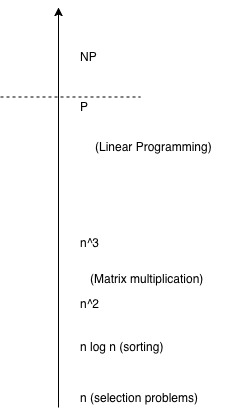
\includegraphics[scale=0.5]{img/laufzeiten}
\end{center}


\subsection{Complexity Analysis of Algorithms: time/space}
\subsubsection{Bubble-Sort}

Array: after (i+1)-step, maximum in A[1...n-i-1]

\begin{verbatim}
Bubblesort(A[1..n])
    for(i=1...n)
        for(j=1...n-i)
            if(A[j+1]<A[j])
                swap(A[j+1],A[j])
\end{verbatim}
Complexity: $\mathcal{O}(n^2)$

\subsection{Space complexity analysis}
Given Graph:
\begin{center}
	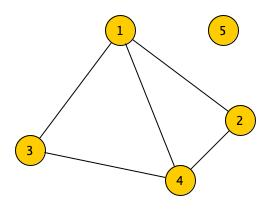
\includegraphics[scale=0.5]{img/graph1}
\end{center}

\subsubsection{Adjacency list}
\begin{center}
	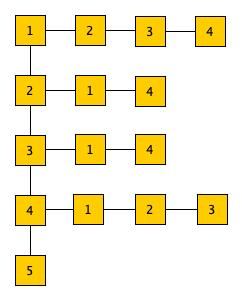
\includegraphics[scale=0.5]{img/adjL1}
\end{center}

Graph has $n$ vertices, $m$ edges. Space requirement: $\mathcal{O}(n \cdot m) \Rightarrow $ Overestimation, holds for full graph, correct answer is $\mathcal{O}(n + m)$.

\subsubsection{Adjacency matrix}

$$\begin{pmatrix}
0 & 1 & 1 & 1 & 0 \\
1 & 0 & 0 & 1 & 0 \\
1 & 0 & 0 & 1 & 0 \\
1 & 1 & 1 & 0 & 0 \\
0 & 0 & 0 & 0 & 0 \\
\end{pmatrix}$$

Entry A[i,j] = 1, if $(i,j) \in E$. On diagonal we see self loops (1). Simple graph has 0s on diagonal. Space requirements: $\mathcal{O}(n^2)$, cause matrix is $ n \times n $ big.

\subsection{Lower bounds}

\paragraph{Input} Array A[1..n]

\paragraph{Output} An Array in sorted form \\

$\exists$ algorithm that sorts in $\mathcal{O}(n\log n)$ time. \paragraph{Question} Can we do better? $\Leftrightarrow \exists$ algorithm to solve the problem in $o(n\log n)$

\fbox{\parbox{\linewidth}{\textbf{Remember:} \\
\begin{itemize}
\item $f = \mathcal{O}(g)$ upper bound $\Leftrightarrow \exists c>0 \exists x_0>0: f(x) \leq c  \cdot g(x) \forall  x \geq x_0$
\item $f = \Omega(g)$ lower bound $\Leftrightarrow \geq$
\item $f = o(g)$ strict upper bound $\Leftrightarrow <$
\item $f = \Theta(g) \Leftrightarrow f = \mathcal{O}(g) \land f = \Omega(g)$
\end{itemize}
}}
Answer: No! Sorting is in $\Omega(n \log n)$. We can simulate any algorithm that sorts an array using comparisons with a decision tree. 

\subsubsection{Example}
A[1],A[2],A[3]. 
\begin{center}
	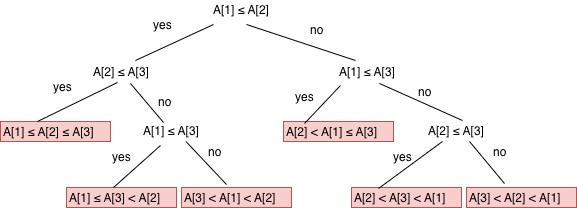
\includegraphics[scale=0.5]{img/decisiontree1}
\end{center}
$\Rightarrow$ We have n numbers, so $\#leaves = n! ( = \#permutations) \Rightarrow$ height of decision tree $\geq \log(n!) = \log(1 \cdot  2 \cdot ...\cdot n/2) \cdot ...) \geq \log(n/2)^{n/2} = \mathcal{O}(n \log n) \Rightarrow $ we need at least $\log(n!)$ comparisons.

\subsection{Mergesort}
\begin{verbatim}
MergeSort(A,l,r)
    if(l = r)
        return A[l]
    m = roundDown((l+r)/2)
    A1 = Mergesort(A,l,m)
    A2 = Mergesort(A, m+l, r)
    B = merge(A1,A2) // O(r-l)
    return B
\end{verbatim}

$$T(n) = \begin{cases} T(\lfloor\frac{n}{2}\rfloor) + T\left( \lceil\frac{n}{2} \rceil\right) + cn & n > 1 \\ 1 & n = 1\end{cases}$$ 
\begin{align*}
n = 2^k \\
T(n) &= 2 T(\frac{n}{2}) + cn  \\
&= 2 (2T(\frac{n}{2^2})+ c \frac{n}{2}) + cn \\
&= ... \\
&= 2^kT(\frac{n}{2^k})+k\cdot c \cdot n = 2^{\log n} T(\frac{n}{2^{\log n}})+ c \cdot \log n \\
&= \mathcal{O}(n \log n)
\end{align*}
With that we have proven, that sorting is in $\Theta(n \log n)$.

\subsection{Convex hull (in computational complexity)}
\paragraph{Input} Points in $\mathbb{R}^2$: $p_1 = (x_1,y_1),...$ 
\paragraph{Output} find a polygon (the smallest one) containing $p_1,...p_n$ \\
$\exists$ many algorithms that solve convex hull in $\mathcal{O}(n \log n)$ time! But: Can we do better = Can we solve the problem in $o(n \log n)$? \\
\paragraph{Idea} CH $\leq o(n \log n)$ sorting (CH is reduced to sorting in the less than $\mathcal{O}(n \log n))$ \\
Instance: $x_1,x_2,...,x_n$ to be sorted. $\Rightarrow$ CH-instance $(x_1,x_1^2),(x_2,x_2^2),...,(x_n,x_n^2)$ (all of them are in CH). The order that appear on CH is a sorting of them (CH-instances drawn look like an exponential function, if sorted by first component). <br>
if CH = $o(n \log n) \Rightarrow$   Sorting = $o(n \log n) \Rightarrow$  that doesn't work with $\Omega(n \log n)$.


\subsection{Example Recursions}

\begin{align*}
	T(n) &= 2 T(\sqrt{n}) + \log n & | m = \log n \\
	T(2^m)&= 2 T(2^{m/2}) + m & | S(m) = T(2^m) \\
	S(m) &= 2 S\left(\frac{m}{2}\right) + m & | \text{from before} \\
	& \in \mathcal{O}(m \cdot \log m) = \mathcal{O}(\log n \cdot \log \log n)
\end{align*}
\begin{align*}
T(n) &= 3T\left(\frac{n}{4}\right)+n \\
&= 3 \left(3 T\left(\frac{n}{16}\right)+\frac{n}{4}\right) +n \\
&= 3^2 T\left(\frac{n}{4^2}\right) + \frac{3}{4}n + n \\
&= 3^2 T\left(3 T \left(\frac{n}{4^3}\right)+\frac{n}{4^3}\right)+ \frac{3}{4}n + n \\
&= 3^3 T\left(\frac{n}{4^3}\right) + \frac{3^2}{4^2}n + \frac{3}{4}n + n \\
&= c \cdot 3^{\log_4(n)} + n \cdot \sum_{i=0}^{\log_4 n-1}\left(\frac{3}{4}\right)^i & | \sum_{i=0}^{\infty} q^i \stackrel{(q<1)}{\rightarrow} \frac{1}{1-q}\\
& \leq  n^{\log_4 3} + n \cdot \frac{1}{1-\frac{3}{4}} & | a^{\log_b n} = n^{\log_b a}; n^1 > n^{\log_43} \\
&= o(n) + 4\cdot n = \mathcal{O}(n)
\end{align*}

\subsection{Logarithmic rules}
\begin{enumerate}
\item $\log a^b = b \log c$
\item $\log(a\cdot b) = \log a+\log b$
\item $x=b ^{\log_bx}$
\item $\log_ax = \frac{\log_bx}{\log_ba}$
\end{enumerate}


\paragraph{Proof} $3^{\log_4n} = n^{\log_43}$
\begin{align*}
	&3^{\log_4n} = n^{\log_43} \\
	&\Leftrightarrow \log_4n = \log_3(n^{\log_43}) & | \text{rule 1}\\
	&\Leftrightarrow  \log_4n = \log_43 \cdot \log_3n \\
	&\Leftrightarrow  \frac{\log_4n}{\log_43} = \log_3n \\
	& \Rightarrow  \text{true with rule 4}
\end{align*}
\begin{flushright}
	$\square$
\end{flushright}

\subsection{One more recursion example}

Given: $A$, $B$, $n \times n$ matrices. $A \times B = C$ \\
Take every matrices and split it into partitions (for example quarters: $\begin{pmatrix}Q1&Q2\\\\Q3&Q4\end{pmatrix}$) but you loose some parts in $C$. But do it more often and combine solutions. For example you have $A_1,A_2,A_3,A_4$ and $B_1,B_2,B_3,B_4$ and we have the Partitions $C_1,C_2,C_3,C_4$ in our solutions matrices. We do it like we had no partitions, so we need to multiply and add the correct Partitions of $A$ and $B$:
\begin{itemize}
\item $C_1 = A_1 \cdot B_1 + A_2 \cdot B_3$
\item  $C_2 = A_1 \cdot B_2 + A_2 \cdot B_4$
\item  $C_3 = A_3 \cdot B_1 + A_4 \cdot B_3$
\item  $C_4 = A_3 \cdot B_2 + A_4 \cdot B_4$
\end{itemize}
That leads to the recursion formula (\textit{irgendwas bisschen komsich aber naja passt so in etwa}): \\

\begin{align*}
T(n) &= 8 \cdot T\left(\frac{n}{2}\right)+\mathcal{O}(n^2) \\
&= 8 \cdot\left(8 \cdot T\left(\frac{n}{2^2}\right) + c\frac{n^2}{2^2} \right) + c \cdot\frac{n^2}{2} \\
&= 8^2 \cdot T\left(\frac{n}{2^2}\right) + c \cdot\frac{8}{2^2}n^2 + c \cdot n^2 \\
&= 8^{\log n} + c \cdot n^2 \cdot\sum_{i=0}^{\log n -1}\left(\frac{8^i}{2^{2i}}\right) & | \sum_{i=0}^{\log n -1}\left(\frac{8^i}{2^{2i}}\right) = \sum_{i=0}^{\log n -1} 2^i = 2^{\log n} -1  \rightarrow  n\\
&= n^{\log_28} + c \cdot n^2 \cdot n \\
&= n^3 +  c  \cdot n^3 = \mathcal{O}(n^3)
\end{align*}

Other way for matricemultiplication: \\
$P_1 = A_1 \cdot (B_2 - B_4)$, $P_2 = B_4 \cdot(A_1-A_2)$,...,$P_7=(A_1-A_3) \cdot (B_1 + B_2)$ \\
$C_1 = P_5 + P_4 - P_2 + P_6$, $C_2=...$,... \\
Recursion formula: $T(n) = 7 \cdot T\left(\frac{n}{2}\right) + \mathcal{O}(n^2)$, so we only have $n^{\log_27} \approx n^{2.8} < n^3$. This is called STRASSEN - schema

\subsection{Analyse complexity/costs with probabilities (average analysis)}

\begin{verbatim}
find_min(Array A)
    min = A[0] //c1
    for(i=1,...n-1)
        if(A[i] < min) //c2
        min = A[i] // c3
    return(min)
\end{verbatim}
Total costs: $c = c_1 + (n-1) \cdot c_2 + (n-1) \cdot c_3$ 

Get probabilities for doing $c_3$: 
$$P(A[1] < A[0]) = \frac{1}{2}$$
$$P(A[2] < min(A[0],A[1])) = \frac{1}{3}$$
$$P(A[i] < min(A[0],...,A[i-1])) = \frac{1}{i+1}$$
Now we can calculate the costs with these probabilities: 
$$X_i = \begin{cases}1 & if(A[i-1]< min(...)) \\\\ 0 & otherwise \end{cases}$$
$$c = c_1 + (n-1) \cdot c_2 + \sum_{i=1}^{n-1}X_i$$
$$E[X_i] = P(X_i = 1) = \frac{1}{i+1}$$
$$E\left[\sum_{i=1}^{n-1}X_i\right] = \sum_{i=1}^{n-1}E[X_i] = \sum_{i=1}^{n-1}\frac{1}{i+1} = \log n$$

\subsection{Armortised Analysis}
Stack $S$ with \texttt{PUSH(x)}($\mathcal{O}(1)$) and \texttt{POP()}($\mathcal{O}(1)$) and \texttt{MULTI-POP(k)} ($\mathcal{O}(min(|S|,k))$) operation. \\
$n$ operations: $\mathcal{O}(n^2)$ because worst operation (`MULTI-POP(k)`) is linear. That's pessimistic. \\
\subsubsection{Accountingmethod}
\begin{tabular}{|c|c|}\hline
	cost & operation \\ \hline
	2 coins & \texttt{push(x)} \\
	0 coins & \texttt{pop()} \\
	0 coins & \texttt{multi-pop(k)} \\ \hline 
\end{tabular} 

$\Rightarrow n$ opertions cost $\leq 2n \Rightarrow \mathcal{O}(n)$

if \texttt{pop()} or \texttt{multi-pop(k)} are applied, at least 1 or $k$ Elements are on the stack $\Rightarrow k$ coins are on the stack.

\subsubsection{Potentialmethod}
"function that describes the bank/the benefit one get doing cheap operations in order to do bad operations" 
\begin{itemize}
\item  $D$ Data structure
\item  $i$ step 
\item  $\Phi$ real value $\geq$ 0
\item $\hat{c_i}$ amortized cost
\item  $c_i$ cost of operation
\item $D_0 \Rightarrow \Phi(D_0) = 0$
\item $D_i (i > 0) \Rightarrow \Phi(D_i) \geq i$

\end{itemize}

$$\hat{c_i} = c_i + \Phi(D_i) - \Phi(D_{i-1})$$

\begin{itemize}
\item \texttt{push(x)} amortized: $1 + |S| + 1 - |S| = 2$
\item  \texttt{pop()} amortized: $1 + |S| - 1 - |S] = 0$
\item  \texttt{multi-pop(k)} amortized: $min(|S|,k) + |S| - min(|S|,k) - |S| = 0$
\end{itemize}

$$\sum_{i=1}^n \hat{c_i}= \sum_{i=1}^n (c_i + \Phi(D_i) - \Phi(D_{i-1}) = \sum_{i=1}^n c_i + \sum_{i=1}^n (\Phi(D_i)-\Phi(D_{i-1})) = \sum_{i=1}^n c_i + \Phi(D_n) [\geq0] - \Phi(D_0)[=0]$$


	\section{MST}

cost/weight function
$w: E \rightarrow \mathbb{N}/\mathbb{R}$

\subsection{Red rule}

$\forall$ cycle colour red the most expensive edge. $\Rightarrow$ the graph without all the red edges is a MST.\\

Search cycle; $m = \#edges, n = \#vertices , m \geq n-1 \Rightarrow  \mathcal{O}(n)$ \\

Selecting max: $\mathcal{O}$(\#vertices in the cycle) = $\mathcal{O}(n)$ \\

How many times do one needs to search in the graph for a cycle: \\ $\mathcal{O}(m-n) = \mathcal{O}(m)$ (until the graph is tree)

$$ \Rightarrow \mathcal{O}(n) \cdot \mathcal{O}(m) = \mathcal{O}(m \cdot n) = \mathcal{O}(n^3)$$

\subsection{Cut-concept}
\begin{center}
	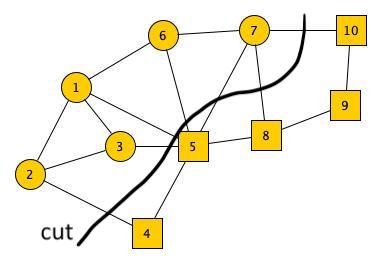
\includegraphics[scale=0.5]{img/graph2}
\end{center}

\begin{itemize}
\item separate the vertices into two sets $V = X \cup X'$, where $X,X'$ are non trivial sets.
\item  all the edges that cut the partition/cross the cut
\item  $\exists$ MST that contains the edge with the minimum weight.
\end{itemize}

\subsection{Blue rule}

$\forall$ cut, colour blue the cheapest edge.

\subsection{Invariant}
$\exists MST(G) T: B \leq T, R \cap T = \emptyset $ \\
$B$ = set of all the blue coloured edges \\
$R$= set of all the red coloured edges

\paragraph{Proof}
base case: $B = \emptyset, R = \emptyset$ holds, because there exists a MST because of all the trees in G, just take the minimum one. Therefore $B \leq T \checkmark, R \cap T = \emptyset \checkmark$ \\

inductive step: \\
RED RULE: edge e \\
in the previous step e is not coloured
\begin{enumerate}
\item edge is not contained in T $\Rightarrow$ Red rule holds
\item edge is contained in T $\Rightarrow$ walk along the cycle and take a edge into T that $w(e') \leq (e)$ $\Rightarrow$ holds
\end{enumerate}

BLUE RULE: edge e \\
was not coloured in the previous step
\begin{enumerate}
	\item e is part of T $\Rightarrow$ Blue rule holds
	\item  e is not part of $T$; $e = (u,v)$, $(u,v)$ were connected with a path and $u \in X$ and $v \in X'$ for every transition along the path $(v' \rightarrow v'') = e'$. $W(e') \geq w(e)$ so it is possible to just take $e$ and leave our $e'$.
\end{enumerate}


\paragraph{COMPLETENESS}
Suppose there is a situation where no rule can be applied to an uncolored edge $e$ \\
blue edges: there is no cycle $\Rightarrow$ blue edges form a forest
\begin{enumerate}
\item  $e$ connects two vertices in the same tree $\Rightarrow$ RED RULE can be applied ($\Rightarrow$ colour it red)
\item $e$ connects two different trees $\Rightarrow$ look at the cut of the two different treefs (B) $\Rightarrow$ BLUE RULE can be applied
\end{enumerate}
There are 7 algorithms that deal with the problem.

\subsection{Kruskal}

Sort the edges in non-decreasing order. Consider the edge next in the order $(u,v)$. \\
if $u$ and $v$ belong to the same subtree $\Rightarrow (u,v)$ red \\
if $u$ and $v$ connect two different subtrees $\Rightarrow (u,v)$ blue

$\mathcal{O}(m \cdot \log m)$
	\section{Minimum Cut Problem }
\paragraph{Input} a graph $G=(V,E,w), W: E \rightarrow \mathbb{R}^+[s\neq t, s,t, \in V]$

\paragraph{Output} a partition of V into S,T (T = V \ S) s.t.

\begin{itemize}
	\item[(i)] $S \neq \emptyset \land T \neq \emptyset [s \in S, t \in T]$
	\item[(ii)] $w(S,T) = \sum_{u\in S, v\in T}w(u,v)$ is minimum over all partitions
\end{itemize}
\begin{center}
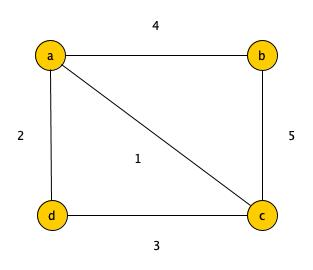
\includegraphics[scale=0.75]{img/graph7} \\
\end{center}
\begin{tabular}{|c|c|} \hline 
	$S$ & $w(S,T)$ \\ \hline 
	a & 7 \\
	b & 9 \\
	c & 9 \\
	\textbf{d} & \textbf{5} \\
	a,b & 8 \\
	b,c &  8 \\
	c,d &  8 \\
	d,a &  8 \\ \hline
\end{tabular} \\

(Max-Cut Problem is NP complete) 

\paragraph{Observation} MinCut $\stackrel{n^2}{\leq}$ Min(s-t)-Cut
$\rightarrow$ can we do better: $\mathcal{o}(n^2)$ \\

\begin{verbatim}
MinCut(G)
min <- infty
for each s in V 
    for each t in V: s != T // two fors -> n^2
        (S,T) <- Min-s-t-Cut(s,t)
        if(S,T) is lighter than min // in Term of weights
            min <- (S,T)
\end{verbatim}

Merging a and b in example \\
\begin{center}
	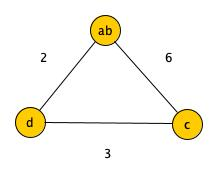
\includegraphics[scale=1]{img/graph8}
\end{center}

Edge ab - c is sum of weight (5 and 1)

\subsubsection{Operation: Merge of two verties}

Given a graph $G = (V,E,w)$ \& $s,t \in V$ , $s \neq t$ the Graph $G\ \{s,t\} = (V',E',w')$ obtained by merging $s,t$. \\

$$V' = V \ \{s,t\} \cup \{X_{s,t}\}$$

$$E' = E \ \{(u,v) \in E: u,v \in \{s,t\}\} \cup \{(X_{s,t},v): (s,v) \in E \lor (t,v) \in E\}$$

$$w'(X_{st},v) = \begin{cases}
w(s,v) & (s,v) \in E \& (t,v) \notin E \\
w(t,v) & (s,v) \notin E \& (t,v) \in  E \\
w(s,v) + w(t,v) & (s,v) \in E \& (t,v) \in E \\
0 & otherwise
\end{cases}$$

\subsection{Theorem 1}

Let $s,t \in V$ of a graph $G = (V,E)$ \& let $G \ \{s,t\}$ be the graph obtained by $G$ by merging $s$ \& $t$.

Then: 
$$min-cut(G) = min\{min-(s,t)-cut(G), minCut(G\ \{s,t\})\}$$


\paragraph{Proof} Let $(S,T)$ be a min cut of $G$ \\ 
$\Rightarrow {s,t} \in \lor \{s,t\} \in T$ [first part] \\
or \\
$s \in S$ \& $t \in T \lor t \in S$ \& $s \in T$ [second part]

\begin{flushright}
	$\square$
\end{flushright}



\begin{verbatim}
n = |V(G)|
if(n=2) return ({v1},{v2})
else let s,t in V, s != t
    (S,T) <- min-(s,t)-cut for G exists algorithm
    (S',T') <- MinGut(G \ {s,t}) // recursion
    return min{(S,T),(S',T')}
\end{verbatim}

Theorem 1 $\Rightarrow$ Correctnes \\

Complexity $\approx (n-1) \cdot c$, where $c$ min-(s,t)-cut(G) \\

\paragraph{Observation} in linear time reduceable $\mathcal{O}(n)$

\subsection{Min-(s,t)-Cur Problem (Stoer \& Wagner)}

\paragraph{Idea}
\begin{itemize}
	\item finds an ordering of the vertices $v_1,..,v_n$, $n = |V(G)|$: ($\{v_1,v_2,...v_{n-1}\},\{v_n\}$) is a min ($v_{n-1},v_n$)-cut
	\item Let $S_i = \{v_1,...,v_i\}$ starting from an arbitrary vertex $v_1$. Then $v_{i+1}$ is selected $s,t$. $w(v_{i+1},S_i) \geq w(v,S_i) \forall v\in V \ S_i$
\end{itemize}



\subsubsection{Example}
\begin{center}
	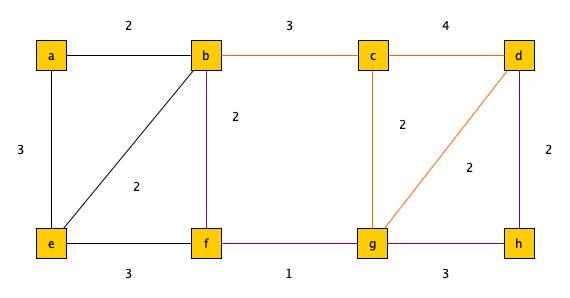
\includegraphics[scale=0.75]{img/graph9}
\end{center}
\begin{tabular}{|c|c|l|}\hline 
	$i$ & $v$ & $S$ \\ \hline 
	1 & b & b \\
	2 & c & b,c \\
	3 & d & b,c,d \\
	4 & g & b,c,d,g \\
	5 & h & b,c,d,g,h \\
	6 & f & b,c,d,g,h,f \\
	7 & e & b,c,d,g,h,f,e \\ \hline 
\end{tabular} \\
$\Rightarrow$ Stoer \& Wagner $(\{a\}, \{b,c,d,g,h,f,e\})$ must be a min (a,e)-cut.

\begin{verbatim}
MinCutPhase(G)
    v1 = any vertex of G
    S = {v1}
    for i = 2 ... n do
        vi <- w({bi},S) >= w({v}, S), v not in V \ S
        S = untion(S, {vi}) // ordered set
    return ({vn},{v1,...,n(n-1)})
\end{verbatim} 
$$\forall v \in V \ S: key(v) = \sum_{v'\in S}w(v,v')$$

$v_{i+1}$ in the vertex with max key

\subsubsection{Fibonacci Heaps}

$\mathcal{O}(Extract-Max) = \mathcal{O}(\log n)$ \\

UpdateKey = $\mathcal{O}(1)$ \\

in total: $|V| \times$ Extract Max and $|E| \times$ UpdateKey $\Rightarrow \mathcal{O}(|V| \log |V| + |E|)$


\subsection{Theroem 2}

$(T,s) = (\{v_1,...,v_{n-1}\}, \{v_n\})$ is a min ($v_{n-1}$, $v_n$)-cut

\paragraph{Proof}

Let $(S,T)$ be any ($v_{n-1},v_n$) cut. We prove: $$w(\{v_1,...mv_{n-1}\}, \{v_n\}) \leq w(S,T)$$
\begin{center}
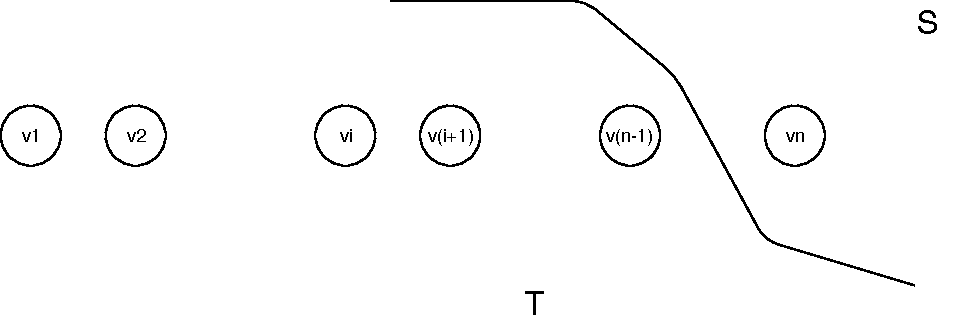
\includegraphics[scale=1]{img/cut}
\end{center}

Critical: $v_i$ is critical iff $\Leftrightarrow (v_i \in S \& v_{i-1} \in T)$ or ($v_i \in T \& v_{i-1} \in S) \Rightarrow v_n \in S \& v_{n-1} \in T$ \\

$A_i := w(\{v_1,..,v_{i-1}\}, \{v_i\}) \leq w(\{v_1,...,v_{i}\} \cap S, \{v_1,...,v_i\}\cap T) =: B_i$ \\

$\forall critical vertex v_i \Rightarrow $ Theorem is proved \\

By induction on the number of critical vertices
\begin{itemize}
\item for the critical vertiex $v_{i_0}:$ \\
\begin{center}
	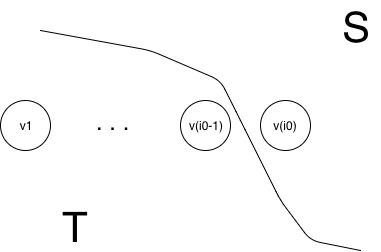
\includegraphics[scale=0.5]{img/cut2}
\end{center}
$\Rightarrow A_{i_0} \leq B_{i_0} \checkmark$  

\item  $A_i \leq B_i$ holds up to the critical vertex $v_i$ [Induction hypothesis]
\item  let $v_j$ be the next critical vertex
\begin{align*}
A_j &= w(\{v_1,...,v_{j-1}\}, \{v_j\}) \\
&= w(\{v_1,...,v_{i-1}\}, \{v_i\}) + w(\{v_1,...,v_{j-1}\}, \{v_j\}) \\
&\stackrel{Stoer+Wagner}{\leq} w(\{v_1,...,v_{i-1}\}, \{v_i\}) + w(\{v_1,...,v_{i-1}\}, \{v_i\}) \\
&\stackrel{IH}{\leq} w(\{v_1,...,v_i\}\cap S,\{v_1,...,v_i\} \cap T) + w(\{v_1,...,v_{j-1}\}, \{v_j\}) \\
&\leq w(\{v_1,...,v_j\}\cap S,\{v_1,...,v_j\}\cap T)
\end{align*}
\begin{flushright}
$\square$
\end{flushright}
\end{itemize}

\paragraph{Claim } 
$w(\{v_1,...,v_{j-1}\},\{v_j\}) \leq w(\{v_1,...,v_{j-1}\} \cap S, \{v_1,...,v_j\}\cap T)$

\paragraph{Proof}
\begin{align*}
w(\{v_1,...,v_{j-1}\},\{v_j\}) &= w(\{v_1,...,v_{i-1}\},\{v_j\}) + w(\{v_i,...,v_{j}\},\{v_j\}) \\
&\stackrel{Stoer+Wagner}{\leq} w(\{v_1,...,v_{i-1}\},\{v_i\}) + w(\{v_i,...,v_{j}\},\{v_j\}) \\
&\stackrel{I.H.}{\leq} w(\{v_1,...,v_{i}\} \cap S, \{v_1,...,v_i\}\cap T) + w(\{v_i,...,v_{j}\},\{v_j\}) \\
&\stackrel{\text{By the fact that vj is critical}}{\leq} w(\{v_1,...,v_{j}\} \cap S, \{v_1,...,v_j\}\cap T) 
\end{align*}

\paragraph{Code}
\begin{verbatim}
MinCut(G)
    n=|V(G)|
    if n = 2 return ({v1},{v2})
    else
        ({v1,...,v(n-1)}{vn}) <- MinCutPhase(G) // V logV+E (Stoer Wagner)
        (S,T) <- MinGut(G\{s,t}) // O(V) (first part in complexity)
        return the lighter of (S,T) and ({v1,...,v(n-1)}{vn})
\end{verbatim} 

\paragraph{Complexity} $\mathcal{O}(V(V \log V+E))$

\subsubsection{Example}

\begin{center}
	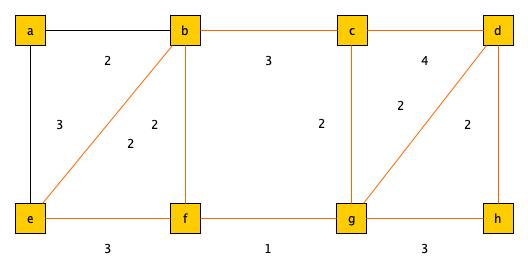
\includegraphics[scale=0.5]{img/graph4}
\end{center}

$v_1$ = b\\
$v_2$ = c\\
$v_3$ = d\\
$v_4$ = g \\
$v_5$ = h \\
$v_6$ = f \\
$v_7$ = e \\
--- \\
$v_8$ = a \\

$\Rightarrow w(\{v_1,...,v_7\},\{v_8\}) = 5$ \\

$\Rightarrow$ merge a and e

\begin{center}
	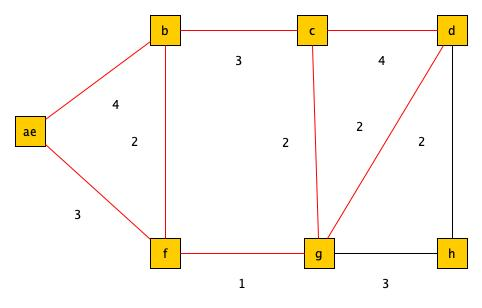
\includegraphics[scale=0.5]{img/graph3}
\end{center}

$v_1$ = b\\
$v_2$ = ae\\
$v_3$ = f\\
$v_4$ = c\\
$v_5$ = d  \\
---  \\
$v_6$ = g \\

$\Rightarrow w(\{v_1,v_2,...,v_6\},^\{v_7\}) = 5$ \\

$\Rightarrow$ merge h and g \\

go on like that.

\newpage
\section{The Max Flow problem}

\paragraph{Input} 
\begin{itemize}
\item  $A$ directed weighted graph (network) $D = (V,E,c)$
\item $c: E \rightarrow  \mathbb{R}^+$ capacity
\item $s,t \in V: s \neq t \& indegree(s) = 0 \& outdegree(t) = 0$
\item $s$: source, $t$: target
\end{itemize}
\begin{center}
	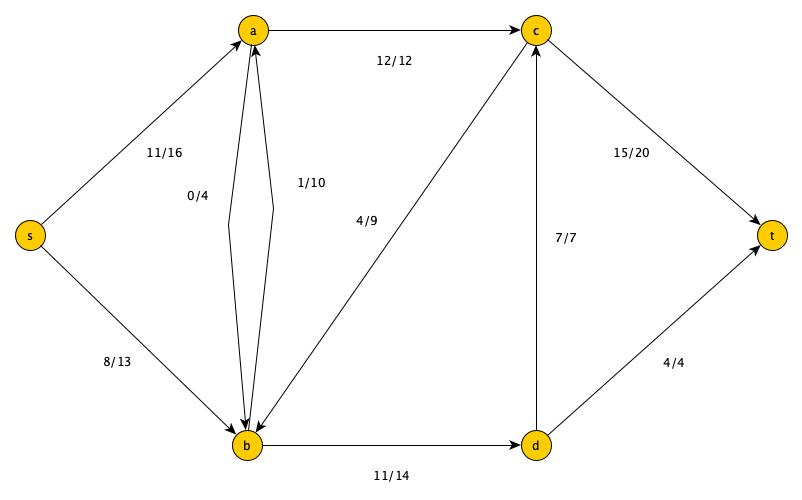
\includegraphics[scale=0.5]{img/graph5}
\end{center}
\textit{Syntax: x/y: x is the flow, y is capacity.} |f| = 19 \\
\textit{Informal: The max quantity of items that can be send from $s$ to $b$ without deviating the capacities \& without storing anything in between.}

\paragraph{Output}
$f: E \rightarrow \mathbb{R}^+$: flow function

\begin{itemize}
\item[(i)] $0 \leq f(u,v) \leq c(u,v) \forall (u,v) \in E$

\item[(ii)] $\sum_{(u,v)\in E}f(u,v) = \sum_{(v,u) \in E}f(v,u) \forall v  \in V \ \{s,t\}$

\item[(iii)] $\sum_{(s,v) \in E} f(s,v)$ is maximized $ (s,v)\in E$ over all flow functions

\end{itemize}

\begin{itemize}
	\item[(i)] called \textbf{capacity constraint}
	
	\item[(ii)] called \textbf{flow consertation}
	
	\item[(iii)] \textbf{called max flow} denoted by $|f^*|$
	
\end{itemize}

\fbox{\parbox{\linewidth}{inflow (flow coming in) and outflow (flow going out) on v}}

\subsection{Example}
\begin{center}
	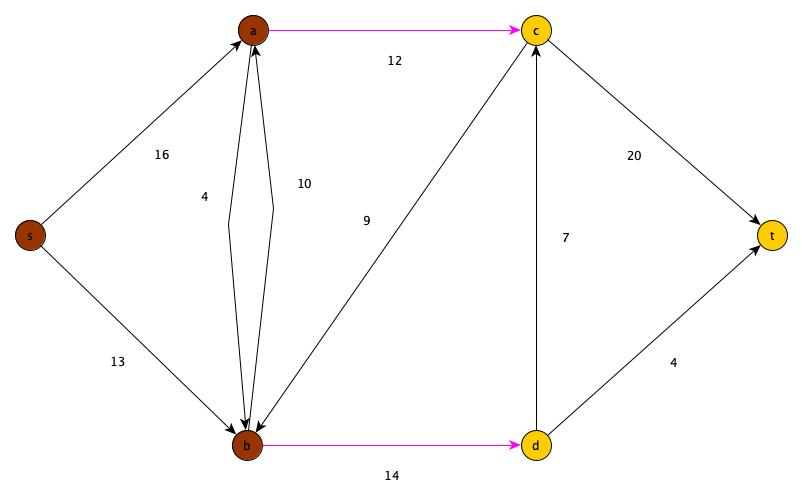
\includegraphics[scale=0.5]{img/graph6}
\end{center}

Cut brown (S) and yellow (T), so $c(S,T) = 26 (= 12+14)$ and
$|l| \leq  c(S,T) \forall  f $


\subsection{Lemma}

$$\forall \text{flow of D} \& \forall cut (S,T): s\in S \& t\in T: |f| \leq c(S,T)$$

\paragraph{Proof}
\begin{align*}
|f| &= \sum_{(s,v)\in E}f(s,v) - \sum_{(v,s)\in E}f(v,s) + \underbrace{\left( \sum_{(u,v)\in E; u\in S\ \{s\}}f(u,v) - \sum_{(u,v)\in E; u\in S\ \{s\}}f(v,u)\right)}_{\text{[0 by (ii)]}} \\
&= \sum_{u\in S} \left( \sum_{(u,v)\in E}f(u,v) - \sum_{(u,v)\in E}f(v,u) \right) \\
& =\underbrace{\left( \sum_{(u,v)\in E/u,v\in S}f(u,v) - \sum_{(u,v)\in E/u,v\in S}f(v,u) \right)}_{\text{[0 by (ii)]}} + \left( \sum_{(u,v)\in E/u\in S,v\in T}f(u,v) - \sum_{(u,v)\in E/u\in S,v\in T}f(v,u) \right) \\
&= \sum_{(u,v)\in E/u\in S,v\in T}f(u,v) - \underbrace{\sum_{(u,v)\in E/u\in S,v\in T}f(v,u)}_{\text{[this part $\geq$ 0 by (i) so cut out]}}
\\
&\leq \sum_{(u,v)\in E/u\in S,v\in T}f(u,v) \stackrel{(i)}{\leq} \sum_{(u,v)\in E/u\in S,v\in T}c(u,v) = c(S,T) 
\end{align*}


\subsection{Corolary 1}

$|f^*| \leq c(S,T) \forall (S,T)$ being an (s,t)-cut

\subsection{Corolary 2}
If there exists a flow f and (s,t)-cut (S,T):

$$|f| = c(S,T) = \sum_{(u,v)\in E,s\in S,v\in T}c(u,v)$$

$$\Rightarrow |f^*| = |f| it's optimal s\in S, v\in T$$


\subsection{Max-flow/min-cut Theorem:}

$$|f^*| is max \Leftrightarrow \exists (s,t)-cut (S,T): |f| = c(S,T)$$

\subsection{Augmenting Path}

$(s,t)$-Path in $D$ align which we can push flow (and augment the flow)

\begin{verbatim}
Ford-Fulkerson (G,s,t)
    initialize f to 0 
    While(esists augmenting path P from s to t)
        Augment f by the bottleneck of P
    return f
\end{verbatim}
\begin{center}
	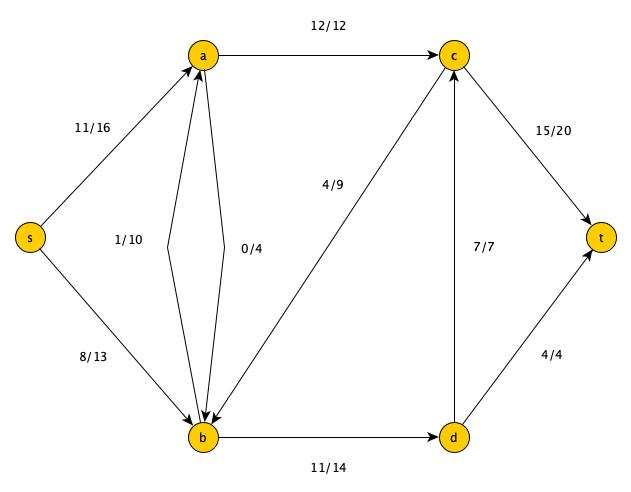
\includegraphics[scale=0.5]{img/graph10}
	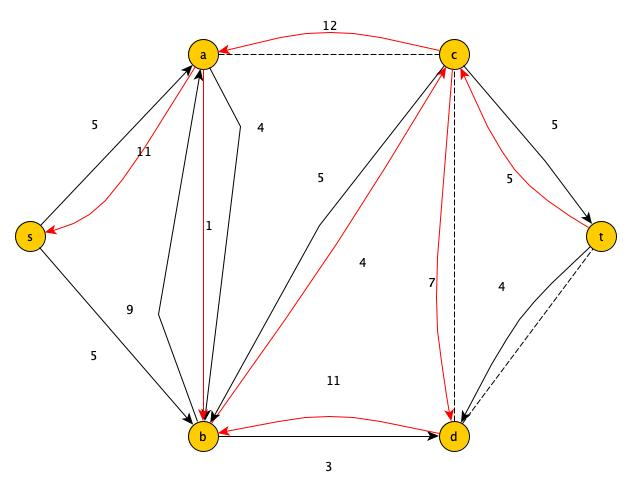
\includegraphics[scale=0.5]{img/graph11}
\end{center}

\subsection{Residual Network}
Describes for every edge $(u,v) \in $E the amount of flow that can be further pushed along $(u,v)$.

$$c_f = (V_f,E_f): 
V_f = V, 
E_f = \{(u,v): c_f(u,v) > 0\},$$$$ 
c_f \text{ residual capacity} \rightarrow 
c_f = \begin{cases} c(u,v)-f(u,v) & (u,v)\in E \\
f(v,u) & (v,u)\in E \\
0 & othehrwise
\end{cases}$$

\begin{center}
	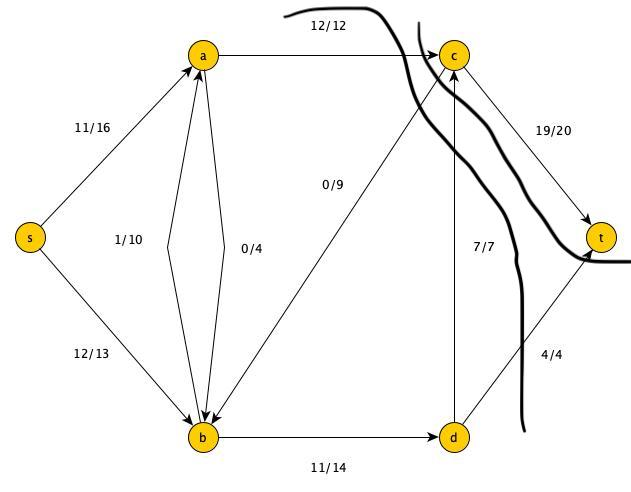
\includegraphics[scale=0.5]{img/graph12}
\end{center}
path: (s,b,c,t), $|f| = 24 > 19, c(S,T) = 24 \Rightarrow f $optimal 

\paragraph{Question} Is the algorithm correct? \\

Augmenting Path Theorem: \\

$f^* \text{ is max flow} \Leftrightarrow \nexists\text{ augmenting path in} G^*_f$ \\

Max-Flow Min-Cut Theorem: \\
$f^*$ is max flow $\Leftrightarrow \exists (s,t)-cut (S_0,T_0), |f^*| = c(S_0,T_0)$

\subsubsection{Theorem}
(i)(ii)(iii) are equivalent: \\
\begin{itemize}
	\item[(i)] $f^*$ is max flow
	
	\item[(ii)] $\nexists$ augmenting path in $G^*_f$
	
	\item[(iii)] $\exists (s,t)-cut (S_0,T_0)$: $|f^*| = c(S_0,T_0)$
	
\end{itemize}
(i) $\Rightarrow$ (ii)$\Leftrightarrow$ $\neg$ (ii) $\Rightarrow \neg$(i) \\
$\neg$(ii) $\Rightarrow \exists$ aug. path $\Rightarrow$ aug. the path $\Rightarrow f^*$ was not max
\begin{flushright}
$\square$
\end{flushright}
(ii) $\Rightarrow$ (iii) \\

\paragraph{Example}
\begin{center}
	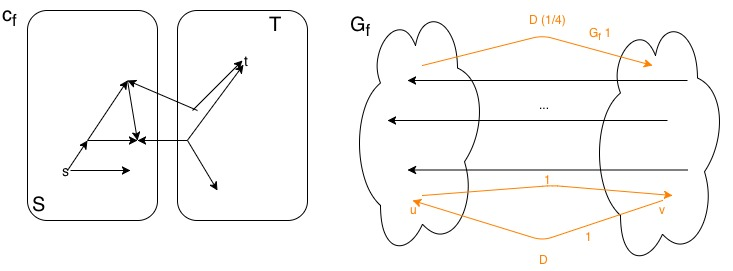
\includegraphics[scale=0.5]{img/graph13}
\end{center}
S: vertices that are reachable by s in $G_f$ \\
T = $V$\ S \\
(ii) $\Rightarrow T \neq  \emptyset (t\in T), (S \neq \emptyset, T \neq \emptyset)$ \\
$|f^*| = ... = \sum_{u,v\in E, u,v\in S}f(u,v)-\sum_{u,v\in E, v,u\in S}f(v,u) + \sum_{u,v\in E, u\in S,v\in T}f(u,v)-\sum_{u,v\in E, u\in S,v\in T}f(v,u)$ \\
$G_p$ s.a. \\
if$(u,v)\in E$ $\Rightarrow f(u,v) = c(u,v)$  full \\
if$(v,u)\in E \Rightarrow f(u,v) = 0$ empty
\begin{flushright}
	$\square$
\end{flushright}

(iii) $\Rightarrow$ (i) \\
see last lecture, follows from the fact that 
$$\forall f \forall (s,t)-cut (S,T): |f| \leq c(S,T)$$

\fbox{\parbox{\linewidth}{If capacities are integers, then $|f^*|$ is also an integer \\ theorem (iii) $|f^*|$ is sum of integers}}



\begin{verbatim}
FordFulkerson(D,s,t)
    for each edge (u,v)\in E // O(|E|)
        f[u,v] <- 0
        flow[u,v] <- 0
    compute G_f // O(|V|+|E|)
    While(exists aug path P from s to t in G_f) // P * O(|E|) oder so aehnlich
        x = min{c_f(u,v): (u,v) in P}
        for earch edge (u,v) in P # O(|E|)
            if(u,v) in E f[u,v] = f[u,v] + x
            if(v,u) in E f[v,u] = f[v,u] - x
            update G_f // O(|V|)
\end{verbatim}

\fbox{\parbox{\linewidth}{if capacities are not integers, then FordFulkersion algorithm may not terminate \\
Assumption: all capacities are integers $\Rightarrow |f^*|$ is integer}}

At each interation the flow is augmenting by at least 1 unit (the augmenting path goes through an edge (u,v): $c_f(u,v)=1$)\\
$\Rightarrow$ While-loop terminates after $|f^*|$ steps \\
$\Rightarrow$ Complexity: $\mathcal{O}(|f^*|\cdot |E|)$ \\

\fbox{\parbox{\linewidth}{1. $\mathcal{O}(|f^*| \cdot |E|)$ depends on the size of the output \\
2. $\exists$ instances that require $\mathcal{O}(|f^*|\cdot |E|)$}} 


\begin{center}
	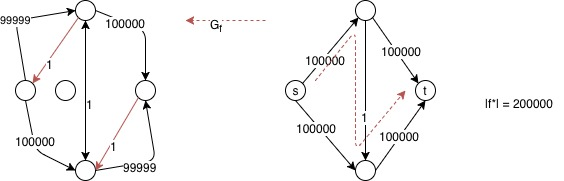
\includegraphics[scale=0.5]{img/graph14}
\end{center}

Can't pass more then max flow on edge. So on more paths the sum still has to be smaller than the max flow on each edge. To calculate max flow efficiently you need to find the min cut. 
\paragraph{Idea} Choose a path from s to t. So how much flow can be passed through that path? $\Rightarrow$ smallest max flow on an individual edge on the path. Push this amount through the path. (At least on edge (with the smallest max flow) is now full). So it translates to the following graph with the capacities $ (u,v) \Rightarrow c(u,v)-f(u,v)$. Non existing edges have capacity 0 and get - the flow the edge in the other direction has. (red in graph): 
\begin{center}
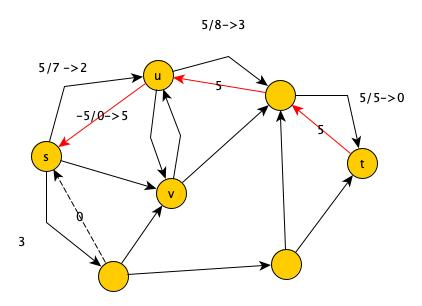
\includegraphics[scale=0.5]{img/graph15} 
\end{center}
Continue with other paths. With the backwards edges the algorithm can tell that the push over this edge was a bad decision by wanting to push over this edge. So we leave the algorithm the freedom to backtrack. \\
Maximum complexity: $\mathcal{O}(|E|\cdot f^*)$. 
\subsection{EdmondKarp}
Search for the shortest path in the Graph ($\#edges$). Augmenting path $s$ to $t$ is the shortest from $s$ to $t$. $\Delta_f(v)$ = min number of edges in $G_f$ from $s$ to $v$. We only need to prove the complexity. (Correctness follows from \texttt{FordFulkerson}) \\
$\mathcal{O}(|V|\cdot |E|^2)$ complexity on \texttt{EdmondKarp}. Wen want to prove that we have $\mathcal{O}(|V|\cdot |E|)$ steps (cause shortest path is $\mathcal{O}(|E|)$.
\paragraph{Proof} At each step there is a bottleneck edge. We want to show that every edge becomes bottleneck once. Because we have more than $|E|$ steps some need to be bottleneck twice. So we prove: \\
$$\forall (u,v): (u,v) \text{ is a BN at most }\mathcal{O}(|V|)\text{ times}$$
We need to state on more property: One edge on the residual network goes to zero (bottleneck). $\Delta_f(w) = |\text{shortest path from s to w in }G_f|$ By changing flow (with the algorithm) we change the network (add and drop edges). By adding an edge there may be a shorter path from $s$ to $w$. \\
We have flow $f$ and after a step we have $f'$ with $\forall w: \Delta_f(w) \leq \Delta_{f'}(w)$. We will prove this first by looking at the contradiction: $\Delta_f(w) > \Delta_{f'}(w)$. 
\begin{itemize}
\item[A:] $\Delta_f(w) > \Delta_{f'}(w) $ [Hy] 
\end{itemize}
$\underbrace{s-...-u-w}_{\text{shortest path}}$ 
\begin{itemize}
\item[B:] $\Delta_f(u) = \Delta_f(w)-1$ 
\item[C:] $\Delta_f(u) \leq \Delta_{f'}(u)$
\end{itemize}
So:
$$\Delta_f(w) = \Delta_f(u)+1 \leq \Delta_{f'}(u)+1 = \Delta_{f'}(w) \Leftrightarrow \Delta_f(w) \leq \Delta_{f'}(w) \; \lightning \text{to [Hy]}$$
So now we know $\Delta_f(w) \leq \Delta_{f'}(w)$. So now we prove 
$$\forall (u,v): (u,v) \text{ is a BN at most }\mathcal{O}(|V|)\text{ times}$$
We can say $\Delta_f(w) \leq |V|$, so $|V|$ is the upper bound.  We have a network with a bottleneck path. At step $i$ the edge $(u,w)$ is the bottleneck so it doesn't exist in step $i+1$. But it exists from $w$ to $u$. On step $j$ it can become bottleneck again but there has to be a step $k$ between $i+1$ and $j$ where the edge $(w,u)$ needs to be bottleneck ($\Rightarrow$ on the shortest path from s to t). So we have the shortest paths: 
$$(i): s-...-u-w-...-t \Rightarrow \Delta_{f_i}(u) = \Delta_{f_i}(w)-1 $$ 
$$(k): s-...-w-u-...-t \Rightarrow \Delta_{f_k}(u) = \Delta_{f_k}(w)+1 $$ 
$$\Delta_{f_i}(w) \leq \Delta_{f_k}(w)$$
$$\Delta_{f_i}(u) = \Delta_{f_i}(w)-1 \leq \Delta_{f_k}(w)-1 = \Delta _{f_k}(u)-1-1$$
Augmentation of at least -2. \\
Because of the upper bound an edge can be bottleneck not more than $\frac{|V|}{2}$ times. $\Rightarrow \mathcal{O}(\frac{|V|}{2} \cdot |E|)$ \\
$\Rightarrow \mathcal{O}(|V| \cdot |E|^2)$ complexity.
\begin{flushright}
	$\square$
\end{flushright}

$|E|$ can me much larger than $|V|$. There is an algorithm that solves Max-Flow in $\mathcal{O}(|V|^2 \cdot |E|)$: \texttt{PUSH-RELABEL} or \texttt{TARJAN-GOLDBERG}. There exist also implementations where you have $\mathcal{O}(|V|^3)$ or $\mathcal{O}(|V|^2\cdot \sqrt{|E|})$. \\
Residual Network is same to EdomdKarp. Difference: you try to do things ore local. On EdmondKarp you always search from $s$ to $t$ $\Rightarrow |E|^2$. \\
Locally you don't know if the flow will reach $t$, so the vertex tries to push the flow to following vertices. If you are lucky this system brings as much flow as possible to $t$. \\
Each vertex has a label, that may change while the algorithm runs (\texttt{relabel}). $s$ will have label $|v|$ and $t$ label $|0|$ all the time. With the algorithm the other labels can change. A vertex can push flow to other vertices if
\begin{enumerate}
	\item There is an edge where you can push (with residual capacity)
	\item The vertex that pushes has a higher label than the vertex that is receiving.
\end{enumerate}
Each step we take one vertex and try to push. So you push to a vertex with lower label and update the capacity on this edge. This you do edge by edge. It can appear that a vertex needs to push flow but has only edges to vertices with higher labels. So the flow gets stuck. So you relabel: You look at the vertices that the vertex could push to and increase the pushing vertex-label to $min(\text{neighbours labels})+1$. You start with every label (except $s$) 0. Then you start pushing from $s$. You won't be able to push more flow than the outgoing capacities on $s$. That is the first upper bound. If somewhere you get stuck and can't go on, try to push it a little bit back. \\
It could happen that $s$ can push as much flow as all the outgoing capacities. So all neighbours of $s$ are now "active". All these vertices has label 0 now. That means they can't push. Relabel one of them to 1. This one tries now to send his received flow. Maybe it has not enough outgoing capacity, so there will be some flow stuck un this vertex, but you don't need to push it back, because $s$ has no capacity left. So the vertex stays active. At some point you give that vertex the label $|v|+1$ to send the flow, that is too much, back to $s$ to say $s$ that this is too much. That happens at the closing part of the algorithm.

\subsection{Matching}
\begin{center}
	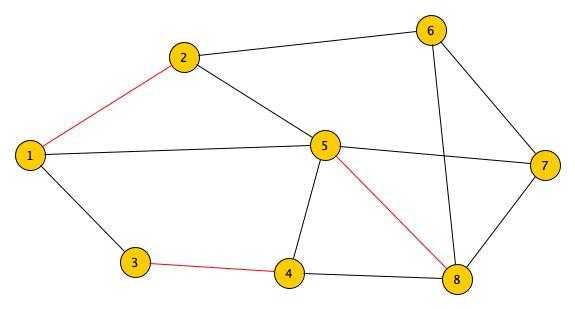
\includegraphics[scale=0.5]{img/graph16}
\end{center}
\paragraph{Matching} On the chosen set of edges there is no common vertex (equivalent to independent set on vertices).
\paragraph{Maximal Matching} There is no edge that can be added without violating the matching constraint. So on the example above only edge $(6,7)$ could be added to get the maximum matching. 
\paragraph{Maximum Matching} The maximum of the maximal matchings. \\
The concept of Max Flow and Maximum Matching is the same. \\
Don't go greedy on Maximum Matching. Usually you want the get the Maximum Matching. \\
We want to find the Maximum Matching in a bipartite graph. Give every edge the capacity 1. Add $s$ at one side with edge (1) to every vertex on that side and equivalent $t$ to the other side. SO at least one edge per vertex on the connecting edges can be taken. SO you search the maximum flow in the graph.
\begin{center}
	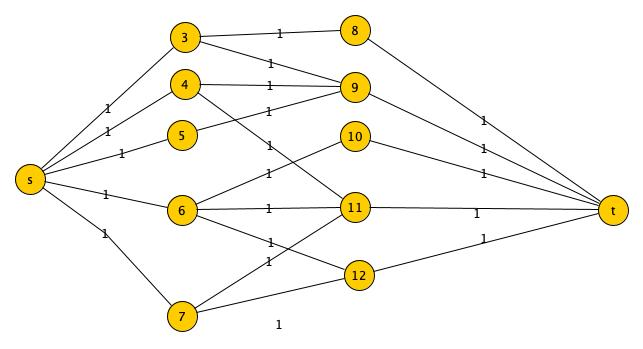
\includegraphics[scale=0.5]{img/graph17}
\end{center}
So to proof:
\begin{enumerate}
	\item If a flow $|f^*|$ exists $\Rightarrow$ matching exists
	\item a max matching exists $\Rightarrow$ a flow $|f^*|$ exists.
\end{enumerate}
	\section{Randomized Algorithms}
\paragraph{Random Algorithm} In the algorithm you compute something random. So on the same input you don't have to get the same output.\\ \\
You can't say, every run gives the optimal solution. But you can get the probability with that you get the optimal solution. \\
\begin{center}
\begin{tabular}{|c|c|c|c|}\hline
	opt. Result & exact Alg & rand Alg (2)& Approx (1)\\ \hline 
	100 & 100 & 100 & 92\\
	100 & 100 & 8& 93\\
	100 & 100 & 90& 99 \\
	100 & 100 & 99& 100 \\
	100 & 100 & 100 & 91\\
	100 & 100 & 100 & 92\\\hline 
\end{tabular}
\end{center}
(1) know that the approximation is very close \\
(2) expect to be very close in p of cases \\


\subsection{Example}
Two Polynomials:
$$P(x) = (x+1)(x-2)(x+3)(x-4)(x+5)(x-6)$$
$$Q(x) = x^6 - 7x^3 + 25$$
$$P(x) \stackrel{?}{\equiv} Q(x)$$
Check $x=2$ ($P$ will evaluate to 0), but
$$Q(2) = 2^6 - 7 \cdot 2^3 + 25 = 33 \neq 0$$
So we can say $P(x) \not \equiv Q(x)$ with $P=1$. \\ If selected number right $\Rightarrow$ $P(x) \not \equiv Q(x)$ with $P < 1$. \\
The random part is to choose $x=2$.  
$$P(x) = x^2 + 7x +1$$
$$Q(x) = (x+2)^2$$
$$P(1) = 1 + 7 + 1 = 9  = (1+2)^2 = Q(1)$$
Choose $x$ from a range of numbers (1...100). \\
Good numbers: $P(x)$ and $Q(x)$ evaluate to different results. \\
Bad numbers: They evaluate to the same result. \\
So how many bad numbers do we have? 
$$F(X) = P(X) - Q(X)$$
If they are equivalent $F$ would evaluate to 0 all the time. The bad numbers are those with $F =$ 0 ($F(3) = P(3) - Q(3) = 0$). Number of bad numbers $\leq d$ where $d$ is the degree of the polynomial. Get a very large range ($d \cdot 100$)so you have many good numbers. So the probability for a bad number is
$$P_{bad} = \frac{d}{100 \cdot d} = \frac{1}{100}$$
One would differentiate between the following two types of randomized algorithms
\begin{itemize}
	\item Monte Carlo: takes polynomial time, gets the right/optimal solution with expected probability
	\item Las Vegas: sure that the right/optimal solution will be found, takes expected polynomial time
\end{itemize}
$$\text{Monte-Carlo} \stackrel{\text{repeat } \infty \text{-many times}}{\rightarrow} \text{Las Vegas}$$
Example from last time: \\
If $\exists x^* P(x^*) \neq Q(x^*) \Rightarrow P(x) \not \equiv Q(x)$\\
$P(x) = x^3 + 2 x^2 - 3x, Q(x) = (x-1)(x^2+2) = x^3+2x-x^2-2$ \\
$P(1) = 0 = Q(1) \Rightarrow $ don't know  whether $P(x) \equiv Q(x)$ \\
$P(2) = 10 \neq 6 = Q(2) \Rightarrow P(x) \not \equiv Q(x) $ \\
Correct answer with some probability. \\
Extract number out of a certain range $[0,100]$. How many good numbers (evaluate to different solutions) and bad (to the same result) are there? \\
Look at: $F(x) = P(x) - Q(x)$ \\
$F(x) = 0 \Leftrightarrow P(x) \equiv Q(x)$ \\
Roots of $F(x)$: "bad numbers" only a few where $F(x) = 0$ \\
\paragraph{Question:} how many "bad numbers" are there? \\
$\Rightarrow$ suppose $deg(Q) = deg(P) = d \Rightarrow d $ bad numbers at most ($\leq d$) \\
Instead of fixed range choose $[0,100 \cdot d]$ \\
$\Rightarrow$ good numbers are $1 - \frac{d}{100d} = 99\%$\\
$\Rightarrow $ increase the range proportionally to $d$ (Monte-Carlo-Algorithm) \\
To increase the probability \\
\begin{itemize}
	\item increase range
	\item repeat the algorithm several times
\end{itemize}
Probability after 2 or $k$ solutions respectively 
$$\frac{1}{100} \cdot \frac{1}{100} = \frac{1}{100^2} \Rightarrow \frac{1	}{100^k}$$
$1-\frac{1}{100^k}$ can make solution arbitrarily close to 1. \\
Also a correct answer is given in one of cases with probability 1 - the "no"-answer. \\
repetition-probabilities for bad numbers
$$\underbrace{\frac{d}{100d} \cdot \frac{d-1}{100d-1} \cdot \frac{d-2}{100d-1}}_{\stackrel{\rightarrow}{\text{prob. gets better/prob. decreases(}\Rightarrow\text{no independent repetitions)}}}$$
if $k>d \Rightarrow \frac{0}{100d-k}$ \\
if $K=d+1$ repetitions the correct solution is found but $\mathcal{O}(d) \cdot d+1 = \mathcal{O}(d^2)$ \\
\paragraph{Complexity} $\mathcal{O}(d\cdot k)$ ($d \rightarrow$ per step, $k \rightarrow$ number of repetitions). \\
Good is $k<<d \Rightarrow$ Complexity stays $\mathcal{O}(d)$ randomization is done to get an efficient algorithm. 
\paragraph{More general formulation} 
conditional probability \\
two events: $w_1,w_2$ \\
independence: $w_1 \Rightarrow Pr(w_1), w_2 \Rightarrow Pr(w_2)$ \\
non-independence: $w_1 \Rightarrow Pr(w_1), w_2 \Rightarrow Pr(w_1|w_2)$ \\
if independence is given $\Rightarrow Pr(w_2) = Pr(w_2|w_1)$ \\
if dependence is given $\Rightarrow Pr(w_2|w_1) = \frac{Pr(w_2 \cap w_1)}{Pr(w_1)}$ \\
events $w_1,w_2$: 
\begin{align*}
P(w_2|w_1) &= \frac{P(w_2 \cap w_1)}{P(w_1)} \\
P(w_1 \cap w_2) &= P(w_2|w_1) \cdot P(w_1) \\
P(w_1 \cap w_2) &= P(w_2) \cdot P(w_1) & | \text{if independent}
\end{align*}
let $w_i := $ get bad numbers at step/repetition $i$
$$P(w_1 \cap w_2 \cap ... \cap w_k) = ?$$ 
correct $W' = 1 -P(w_1 \cap w_2 \cap ... \cap w_k)$
\begin{align*}
	P(w_1 \cap w_2 \cap ... \cap w_k) &= P(w_k|w_{k-1} \cap ... \cap w_1) \cdot P(w_1 \cap ... \cap w_{k-1}) \\
	&= P(w_k|w_{k-1} \cap ... \cap w_1) P(w_{k-1}|w_{k-1} \cap ... \cap w_1) \cdot P(w_1 \cap ... \cap w_{k-2}) \\
	&= \left( \prod_{i=2}^{k} \left(P|w_1 \cap ... \cap w_{i-1} \right) \right) \cdot P(w_1)
\end{align*}
\subsection{Random Walk}
Search space 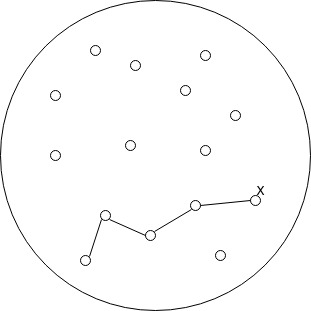
\includegraphics[scale=0.2]{randomizedAlg/opt-way.jpg} optimal Solution \\
do from every point a random choice and walk down the chosen path \\
$-n-...-\stackrel{you}{\underbrace{0}_{0.5 \leftarrow \rightarrow 0.5}}------------------\stackrel{\times}{n}$ \\
Probability of doing a step with $\frac{1}{p}$ and $1-\frac{1}{p}$ in the other direction. Want to estimate $\# steps$ to reach $n$. $w: $ event $you$ reaches $\times$, $Pr(w)=?$ \\
$Z:$ random variable = $\# steps$ before reaching $\times$ \\
Try to compute the expected value 
\begin{align*}
	E[Z] &= ? \\
	E[Z] &= \sum_i(i \cdot P(Z=i)) & |i \in \{\text{values $Z$ can take}\}
\end{align*}
\paragraph{Example} dice \\
$Z = $ numbers on dice 
\begin{align*}
E(Z) &= \frac{1}{6} \cdot 1 + \frac{1}{6} \cdot 2 + \frac{1}{6} \cdot 3 + \frac{1}{6} \cdot  4 + \frac{1}{6} \cdot 5 + \frac{1}{6} \cdot 6 \\
&= 1 \cdot P(Z=1) + 2 \cdot P(Z=2) + ... + 6 \cdot P(Z=6) \\
&= 3.5
\end{align*}

\subsubsection{Random Walker} $0--------(i-1)\stackrel{\leftarrow}{-}\stackrel{\mathwitch}{i}\stackrel{\rightarrow}{-}(i+1)---------n-\rightarrow $ \\
$Pr(i \rightarrow i+1) = \frac{1}{2}$, $Pr(i \rightarrow i-1) = \frac{1}{2}$ \\
Initially $\mathwitch$ is at position 0. $\rightarrow$ What is the expected number of steps that $\mathwitch$ needs to reach $n$? \\
$X_i$ the random variable that corresponds to the number of moves that $\mathwitch$ needs to reach $i$. Find $E[X_n]$. Sei $T(i) = E(X_i)$ \\
\begin{align*}
	t(0) &= 0 \\
	t(1) &= 1 + \frac{1}{2} \cdot t(0) + \frac{1}{2} \cdot t(2) \\
	&... \\
	t(i) &= 1 + \frac{1}{2} \cdot t(i-1) + \frac{1}{2} \cdot t(i+1) \\
	&... \\
	t(n-1) &= 1 + \frac{1}{2} \cdot t(n-2) + \frac{1}{2} \cdot t(n) \\
	t(n) &= 1 + \frac{1}{2} \cdot t(n-1) & |unique
\end{align*}
\begin{center}
    $\left.\begin{aligned}
t(n-1) = 1 + \frac{1}{2} \cdot t(n-2) + \frac{1}{2} (1 + \cdot t(n-1)) \\
\Leftrightarrow \frac{1}{2} t(n-1) = \frac{3}{2} +  \frac{1}{2}t(n-2) \\
\Leftrightarrow t(n-1) = 3 + t(n-2) \\ \phantom{t} \\ 
t(n-2) = 1+\frac{1}{2}t(n-3) + \frac{1}{2} (3+t(n-2)) \\
\Leftrightarrow \frac{1}{2}t(n-2) = \frac{5}{2} + \frac{1}{2} t(n-3) \\
\Leftrightarrow t(n-2) = 5 + t(n-3) \\ ... \\
t(n-i) = 1 + 2i + t(n-i-1) \\
t(1) = 1 + 2 (n-1) + t(0) = 1 + 2(n-1)
\end{aligned}\right\rbrace$Backward-Propagation
\end{center}
\begin{center}
	$\left.\begin{aligned}
	t(1) = 1 + 2(n-1) \\
	t(2) = 1 + 2(n-1) + 1 + 2(n-1)  \\ = 3 + 2((n-1)+(n-2)) \\
	... \\
	t(n) = n + 2((n-1)+(n-2)+...+0) \\
	= n+2 \frac{(n-1)n}{2}  \\= n + n^2 - n = n^2
	\end{aligned}\right\rbrace$Forward-Propagation
\end{center}

\subsubsection{2-SAT}
\paragraph{Input} A logical formula $\Phi$ with $n$ variables and $m$ clauses each with 2 literals
\paragraph{Example} $\Phi = (x_1 \lor \overline{x_2}) \land (\overline{x_2} \lor \overline{x_3}) \land (x_1 \lor x_2) \land (\overline{x_1} \lor \overline{x_4})$
\paragraph{Output} An assignment of the truth values of each variable of $\Phi$ that make $\Phi$ satisfiable.
\paragraph{Example} $x_1=true;x_3=false;x_4=false,x_2=true$
\paragraph{A randomized algorithm} 
\begin{verbatim}
Start with arbitrary assignment (e.g. xi = false forall i=1,...,n) 
while(exists an unsatisfied clause ) [or tired flipping coins]
  c <- some unsatisfied clause
  choose a variable of c by flipping a coind
  change the value of the variable
\end{verbatim}
\paragraph{Example} $x_1=x_2=x_3=x_4=false$ \\
$(x_1 \lor x_2)$ chosen $\rightarrow x_2=true$ \\
$(x_1 \lor \overline{x_2})$ chosen $\rightarrow x_2=false$ \\
... \\
$\mathwitch -----------------------------S-----\rightarrow$ \\
What is $Pr \rightarrow ?$, What is $Pr \leftarrow ?$ \\
$S \leftarrow$ a (any) truth assignment of $\Phi$ \\
$A_j \leftarrow$ the assignment of values to the variables of $\Phi$ after the $j$-th iteration \\
$X_i \leftarrow$ the number of variables that have the same value in $A_j$ and $S$. \\
If $X_j = n \Rightarrow S=A_j$ \\
$\left.\begin{aligned}
S = x_1 = t, x_3=t,x_4=f, x_2 = t \\
A_0=x_1=x_2=x_3=x_4=f
\end{aligned}\right\rbrace X_0=2$ 
$x_0:$ How many do the two sets have in common ($X_j=(A_j\cap S)$) 
\paragraph{Claim} If $\Phi$ has a truth assignment $S$ making it true, then in $n^2$ iterations the algorithm is expected to find $S$.
\subparagraph{Proof}$\mathwitch --------------------------S(X_j=n)-----\rightarrow$ \\
Wlog ("without loss of generality") $X_0 = 0$ \\
What is the probability that at some iteration $j$ $\mathwitch$ moves closer/further away from $S$? \\
$Pr(X_{j+1} = k+1|X_{j=k}) \rightarrow \mathwitch$ moves closer \\ 
$Pr(X_{j+1} = k-1|X_{j=k}) \rightarrow \mathwitch$ moves away \\
$(x_k,x_{\lambda}) \rightarrow $ the unsatisfied clause of the $j$-th iteration \\
$\rightarrow$ \textit{Observation: $(x_k,x_{\lambda})$ cannot have the same value as $S$. At least one of the $x_k,x_{\lambda}$ must have a different value in $S_i$, otherwise $(x_k,x_{\lambda})$ satisfied}
\begin{itemize}
	\item Both have different values: $P(closer) = 1$
	\item Exactly one has a different value: $P(closer) = \frac{1}{2} = P(away)$
\end{itemize}
\paragraph{Theorem} If the algorithm makes $sn^2$ iterations and $S$ is satisfiable, then $Pr(\text{not finding }S) \leq \frac{1}{2}$
\subparagraph{Proof} $X \leftarrow$ random variable that corresponds to the number of iterations to find $S \stackrel{\text{Random\\Walker}}{\Rightarrow} E(X) = n^2$ \\
$Pr(\text{not finding S}) = Pr(X > 2n^2) \stackrel{Markov Inequality}{\leq} \frac{E[X]}{2n^2} ) = \frac{1}{2}$ 
\paragraph{Markov Inequality} $Pr(X \geq \alpha) \leq \frac{E(X)}{\alpha}$
\subparagraph{Proof} 
\begin{align*}
	E(X) &= \sum_{i=0}^{\infty}Pr(X=i) \\
	&= \underbrace{\sum_{i\geq\alpha} iPr(X=i)}_{\geq 0} + \underbrace{\sum_{i<\alpha}iPr(X=i)}_{\geq 0} \\
	&\Rightarrow E(X) \geq \sum_{i \geq \alpha}iPr(X=i) \geq \alpha \sum_{I \geq \alpha}Pr(X=i)
\end{align*}
\paragraph{2-SAT is in P} $\Phi = (\overline{x} \lor y) \land (\overline{\text{\textcolor{orange}{$y$}}} \lor \text{\textcolor{orange}{$z$}}) \land (\text{\textcolor{red}{$z$}} \lor \text{\textcolor{red}{$y$}})$ \\
$x \lor y \Leftrightarrow \overline{x} \Rightarrow y \Leftrightarrow \overline{y} \Rightarrow x$ \\
Based $\Phi$ creates a graph $G_{\Phi}$: $\forall$ variable $x \in \Phi$, $G_{\phi}$ has two vertices $x, \overline{x}$ \\
example $G_{\Phi}:$ \\
\begin{center}
	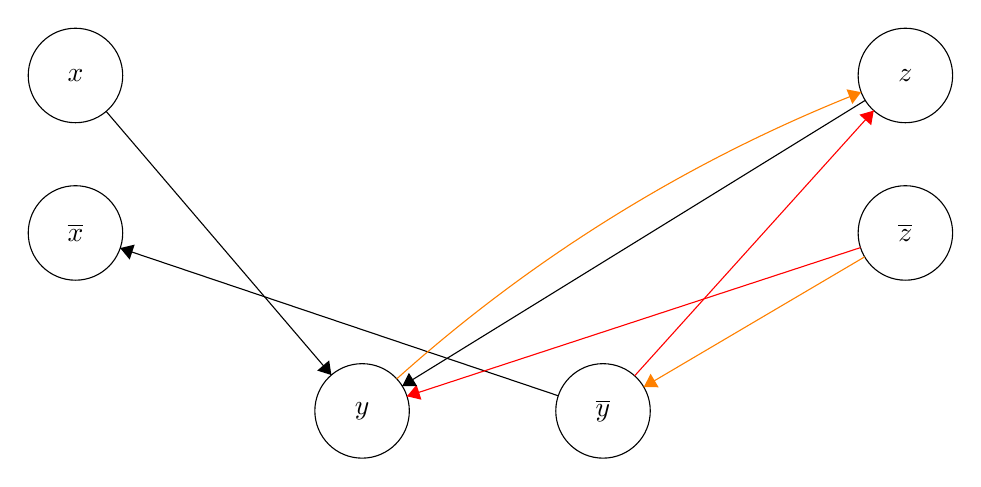
\begin{tikzpicture}[scale=0.2]
	\tikzstyle{every node}+=[inner sep=0pt]
	\draw [black] (9.3,-24.7) circle (3);
	\draw (9.3,-24.7) node {$x$};
	\draw [black] (9.3,-34.7) circle (3);
	\draw (9.3,-34.7) node {$\overline{x}$};
	\draw [black] (27.5,-46) circle (3);
	\draw (27.5,-46) node {$y$};
	\draw [black] (42.8,-46) circle (3);
	\draw (42.8,-46) node {$\overline{y}$};
	\draw [black] (62,-24.7) circle (3);
	\draw (62,-24.7) node {$z$};
	\draw [black] (62,-34.7) circle (3);
	\draw (62,-34.7) node {$\overline{z}$};
	\draw [black] (11.25,-26.98) -- (25.55,-43.72);
	\fill [black] (25.55,-43.72) -- (25.41,-42.79) -- (24.65,-43.44);
	\draw [black] (39.96,-45.04) -- (12.14,-35.66);
	\fill [black] (12.14,-35.66) -- (12.74,-36.39) -- (13.06,-35.44);
	\draw [orange] (59.41,-36.22) -- (45.39,-44.48);
	\fill [orange] (45.39,-44.48) -- (46.33,-44.5) -- (45.82,-43.64);
	\draw [orange] (29.702,-43.963) arc (131.89631:111.48533:97.804);
	\fill [orange] (59.19,-25.76) -- (58.26,-25.58) -- (58.63,-26.51);
	\draw [red] (59.15,-35.63) -- (30.35,-45.07);
	\fill [red] (30.35,-45.07) -- (31.27,-45.29) -- (30.96,-44.34);
	\draw [black] (59.45,-26.28) -- (30.05,-44.42);
	\fill [black] (30.05,-44.42) -- (31,-44.43) -- (30.47,-43.58);
	\draw [red] (44.81,-43.77) -- (59.99,-26.93);
	\fill [red] (59.99,-26.93) -- (59.08,-27.19) -- (59.83,-27.86);
	\end{tikzpicture}
\end{center}
$\forall$ clause $(x \lor y)$ has two edges $\overline{x} \rightarrow y$, $\overline{y} \rightarrow x$
\paragraph{Theorem:} $\Phi$ is unsatisfiable $\Leftrightarrow$ $\exists$ variable $x$ in $\Phi$:$x \stackrel{P_1}{\leadsto} \overline{x}$ and $\overline{x} \stackrel{P_2}{\leadsto}x$ in $G_{\Phi}$.
\subparagraph{Proof:} $(\Leftrightarrow)$: 
\begin{center}
	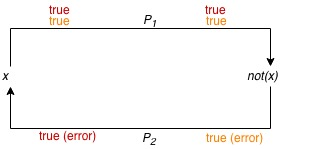
\includegraphics[scale=0.75]{img/proof422}
\end{center}
Assume $\Phi$ is unsatisfiable. \\
$(\Rightarrow)$: If there exsit paths $P_1$ and $P_2$ then $\Phi$ is unsatisfiable. \\
Assume $\Phi$ is satisfiable. \\
$x\stackrel{\text{\textcolor{red}{T}}}{x} \underbrace{\rightarrow \cdot \rightarrow \cdot \rightarrow}_{\text{\textcolor{red}{$\tau$}}} \underbrace{a ... b \rightarrow}_{\text{\textcolor{red}{F}}} \stackrel{\text{\textcolor{red}{F}}}{\overline{x}}$ \\
$a$ true, $b$ false, $\overline{a} \lor b = $false $\lightning$. \\
String connected components: \\
If there is a component which contains $x$ ad $\overline{x}$ then $\Phi$ is unsatisfiable.

\subsection{Convex hull}
\paragraph{Input} $n$ points $P = \{p_1,p_2,...,p_n\}, p_i = (x,y) \in \mathbb{R}^2$. \textit{in general position}
\begin{itemize}
	\item[(i)] no three points on a line
	\item[(ii)] no two points on a vertical line $\Rightarrow x_i \neq x_j \forall i \neq j$
\end{itemize}
\paragraph{Output} The smallest convex hull polygon $Q$ that contains all points, i.e. $P \subseteq Q$ \\
\textit{$Q$ is convex $\Leftrightarrow \forall p,q \in Q: \overline{pq}\in Q \Leftrightarrow$ all angels of $Q$ are $\leq 180^{\circ}$}
\subsubsection{Example}
\begin{center}
	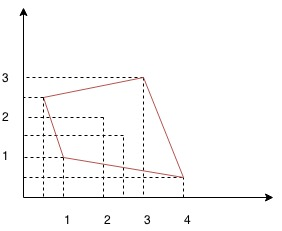
\includegraphics[scale=1]{img/convex} 
\end{center}
\paragraph{Recall} Convex Hull $\in o(n \log n)$, Convex Hull $\geq_n$ Sorting \\
\subsubsection{Convex hull representation}
\begin{center}
	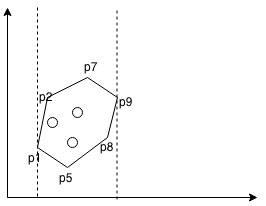
\includegraphics[scale=0.5]{img/convex1} 
\end{center}
The points of CH in clockwise (ccw) order around the boundary. $\underbrace{p_1}_{leftmost},p_2,p_7,p_9,p_8,p_5$
\paragraph{Observation} The leftmost, rightmost, topmost, bottommost points belong to the convex hull. \\
\begin{center}
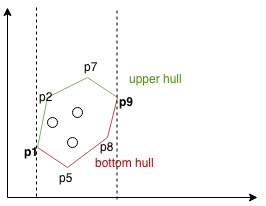
\includegraphics[scale=0.5]{img/convex2} 
\end{center}
\subsubsection{Incremental algorithm} to compute upper (bottom) hull. (\textit{incremental: processes on point at each step}). Points are sorted left to right!
\paragraph{Invariant} For the first $i-1$ points, the upper hull has benn computed. \\
\begin{center}
	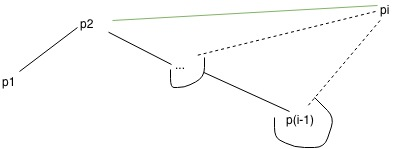
\includegraphics[scale=0.5]{img/convex3} 
\end{center}
Angle at $p_{i-1}$ too big, so pop $p_{i-1}$ from stack. $p_{...}$ angle too big, so pop $p_{...}$ from stack. $p_2$ is ok so let it on the stack and push $p_i$.
\subparagraph{Pseudo code}
\begin{verbatim}
Sort the points L -> R: p1,...,pn // O(n log n)
push (p1, H)
push (p2, H)
for i=3 to n // O(n)
    while (|H| >= 2 & < (pi, first(H),second(H)) > 180grad)
        pop(H)
    push(p1, H)
\end{verbatim}
\subparagraph{Correctness} $p_i \in $ Upper hull (rightmost); the removed point $\notin$ Upper hull
\subparagraph{Complexity} $\#push/pop \in \mathcal{O}(n)$ (can't pop more than we have pushed)
\subsubsection{Randomised incremental Construction (RIC)}
\begin{enumerate}
	\item shuffle points: $P_1,...,P_n$ (randomisation): $S_i = \{p_1,...,p_i\}$ \\
	\begin{center}
		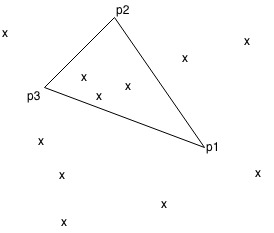
\includegraphics[scale=0.5]{img/convex4} 
	\end{center}
	\item $conv(S_3) \leftarrow$ convex hull of $p_1,p_2,p_3$ 
	\item $p_0 \leftarrow$ in $conv(S_3)$
	\item Draw an arc from $p_0$ to $\forall p \in P \backslash S_3$
	\begin{center}
		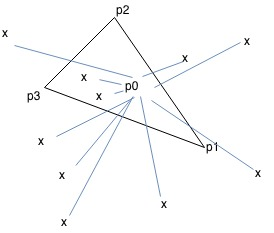
\includegraphics[scale=0.5]{img/convex5} 
	\end{center}
\item The conflict list of each edge $e$ of $conv(S_3)$ consits of all points of $P \backslash S_3$ whose arc crosses $e$ 
\begin{center}
	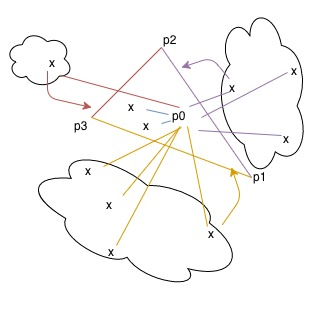
\includegraphics[scale=0.5]{img/convex6} 
\end{center}
\item The points of $P \backslash S_3$ that are not in any conflict lists $\rightarrow$ inactive
\end{enumerate}
\paragraph{Invariant(s)} for the first $i-1$ points 
\begin{itemize}
	\item $conv(S_{i-1})$: convex hull of $S_{i-1}$
	\item each edge of $conv(S_{i-1})$ has a conflict list of active points
	\begin{center}
		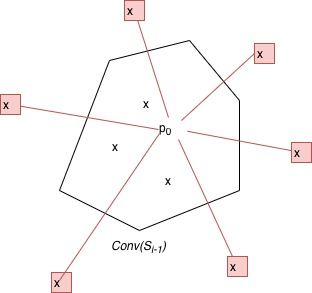
\includegraphics[scale=0.5]{img/convex7} 
	\end{center}
	\item each point in $P \backslash S_{i-1}$  that is active is associated with an edge of $conv(S_{i-1})$
		\begin{center}
		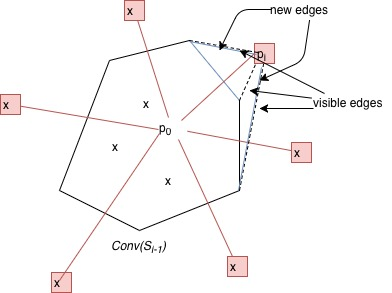
\includegraphics[scale=0.5]{img/convex8} 
	\end{center}
\end{itemize}
\begin{verbatim}
for i=4 ...n
    if pi is active
        e <- associated with pi
        (S1) go left & right on conv(S_{i-1}) to find the visible edges from pi
        (S2) replace the visible edges with two new edges incident to pi
        (S3) "move" th epoints in the conflict lost of the visible edges to 
          the new edge /filter for inactive/active
    else conv(S_i) = conv(S_{i-1})
\end{verbatim}
\subparagraph{Complexity} Steps 1 (S1) \& 2 (S2): $\mathcal{O}(n)$ in total. Each time we add two edges and to remove an edge it must have been added first. 
$$\#removals \leq 2\#additions \in \mathcal{O}(n)$$
Step 3 (S3): $\mathcal{O}(n^2)$ is straight-forward. \\ 
\textbf{Backward Analysis:} $S_i \rightarrow S_{i-1}$ \\
\begin{align*}
E(\#ofPointerUpdates) &= \sum_{e \in conv(S_i)}(\text{size of conf. list of }e) \cdot \underbrace{Pr(e\text{ is removed})}_{\frac{2}{i}} \\
&= \frac{2}{i} \sum_{e \in conv(S_i)}(\text{size of conf. list of }e) \\ &= \frac{n}{i} \\
&\Rightarrow E(\text{overall pointer update}) = \sum_{i = 1}^{n} \frac{n}{i}\\ &= n \cdot \sum_{i = 1}^{n} \frac{1}{i} = \mathcal{O}(n \log n) & |\text{Harmonic sequence}
\end{align*}
\subsection{Unweighed Min-Cur Problem}
\paragraph{Input} a graph $G = (V,E)$
\paragraph{Output} a partition of $V$ into $S,T$:
\begin{itemize}
	\item $S \cup T = V \& S \cap T = \emptyset$
	\item $S \neq \emptyset \neq T$
	\item $w(S,T) = \#edges \equiv | \{(u,v) \in E: u \in S \& v \in T \}|$ is minimum over all partitions of $V$. 
\end{itemize}
\paragraph{Example}
\begin{center}
	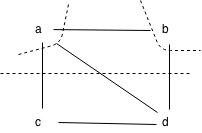
\includegraphics[scale=0.75]{img/ex435} \\ \vspace*{0.5cm}
\begin{tabular}{ccc} \hline \hline 
	$S$ & $T$ & $w(S,T)$ \\ \hline 
	a & b,c,d & 3 \\
	b & a,c,d & 2 \\
	c & a,b,d & 3 \\
	d & a,b,c & 2 \\
	ab & c,d & 3 \\
	... & ... & ...  \\\hline
\end{tabular}
\end{center}
\subsubsection{Stoer \& Wagner} $\mathcal{O}(|V|(|V|\log|V|+|E|))$ \\
\paragraph{Question} Can we do better? \\
\subsubsection{A randomized algorithm}
\begin{verbatim}
Repeat n-2 times the following
  1) Pick an edge (u,v) uniformly at random
  2) Merge(*) the two endpoints of (u,v) into a supernode
G has only two supernodes: v1,v2
Return(S(v1),S(v2)) //S(vi) = {v in V: v was merged to Vi} i = 1,2
\end{verbatim}
(*) Replace by supernode, Remove self-loops, keep parallel edges. \\
\begin{center} 
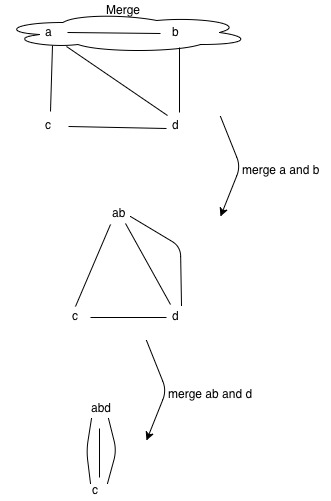
\includegraphics[scale=0.75]{img/sw435}
\end{center}
\textbf{Idea:} Unlikely that (u,v) is in $MinCut(S^*,T^*)$ \\
\paragraph{Lemma 1} If $(S^*,T^*)$ is a min-cut, then the $w(S^*,T^*) \leq \deg(v) \forall v \in V$
\subparagraph{Proof} Assume $\exists v_0 \in V: \deg(v_0) < w(S^*,T^*)$ (*1) \\
new graph: \\
\begin{center} 
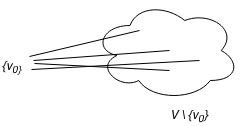
\includegraphics[scale=0.75]{img/graph18}
\end{center} 
Define cut $(A,B): A= \{v_0\}, B= V \backslash \{v_0\}$ \\
$w(A,B) = \deg(v_0) \stackrel{(*1)}{<} w(S^*,T^*) \lightning$
\begin{flushright}
	$\square$
\end{flushright} 
\paragraph{Corollary} $|E| \geq \frac{n}{2}\underbrace{w(S^*,T^*)}_{minCut}$
\subparagraph{Proof}
\begin{align*}
	2 \cdot |E| &= \sum_{v \in V}\deg(v) \\
	&\stackrel{\text{Lemma 1}}{\geq} \sum_{v \in V} w(S^*,T^*) \\
	&= n \cdot w(S^*,T^*) \\
	&\Rightarrow |E| \geq \frac{n}{2} w(S^*,T^*)
\end{align*}
\begin{flushright}
	$\square$
\end{flushright}
\paragraph{Theorem} The randomized algorithm return s a min-cut with probability $\geq \frac{2}{n^2}$
\subparagraph{Proof} $G_j \leftarrow$ the graph obtained after the $j$-th iteration with $n_j = n$ \\
$A_j \leftarrow$ the event that no edge of $(S^*,T^*)$ is selected at this iteration\\
$Pr(\text{algorithm return a min-cut}) = Pr(A_1 \cap A_2 \cap ... \cap A_{n-2})$ 
$=Pr(A_1) \cdot Pr(A_2|A_1) \cdot \cdot \cdot Pr(A_{n-2}|A_1 \cap ... \cap A_{n-2})$ \\
$Pr(A_1) = 1 - Pr(\text{an edge of }(S^*,T^*) \text{ is selected in the first iteration}) = 1- \frac{w(S^*,T^*)}{|E|}$ (Corollary 1) \\
$|E| \geq \frac{n}{2}w(S^*,T^*) \Leftrightarrow \frac{2}{n} \geq \frac{w(S^*,T^*)}{|E|} \Leftrightarrow 1 - \frac{w(S^*,T^*)}{|E|} \geq 1 - \frac{2}{n}$ \\
$\Rightarrow 1 - \frac{w(S^*,T^*)}{|E|} \geq 1 - \frac{n}{2} = \frac{n-2}{n}$ independent of $|E|$ \\
$Pr(A_2|A_1) = ...  \geq \frac{n_1-2}{n_1} \stackrel{n_1=n-1}{=} \frac{n-1-2}{n-1} = \frac{n-3}{n-1} $ \\
$Pr(A_j|A_1 \cap ... \cap A_{j-1}) \geq \frac{n-j-2}{n-j}$ \\
$Pr(\text{algorithm returns min-cut}) = \frac{n-2}{n} \cdot  \frac{n-3}{n-1} \cdot \frac{n-4}{n-2} \cdot ... \frac{2}{4} \cdot \frac{1}{3} = \frac{2}{n(n-1)} \geq \frac{2}{n^2}$
\begin{flushright}
	$\square$
\end{flushright}
\paragraph{Corollary 2} If we repeat the algorithm $n^2 \ln n$ times, then the probability of not reporting the min-cut is $\leq \frac{1}{n^2}$
\subparagraph{Proof}
\begin{align*}
	Pr(\text{not reporting the min-cut}) &= (1-\frac{2}{n^2})^{n^2 \ln n} \\
	&=\left[ \left( 1- \frac{2}{n^2}\right)^{\frac{1}{2}n^2} \right]^{2 \ln n} &| (1-\frac{1}{x})^x \leq \frac{1}{e} \text{Monte Carlo}\\
	&\leq \left( \frac{1}{e} \right)^{2 \ln n} \\
	&= (e^{\ln n})^{-2} = n^{-2} = \frac{1}{n^2} 
\end{align*}
\begin{flushright}
	$\square$
\end{flushright}
\fbox{\parbox{\linewidth}{Note: If we repeat randomized algorithm $n^2 \ln n = \Theta(n^2 \log n)$ then the $Pr(\text{not reporting a solution correct}) \leq \frac{1}{n^2}$}} 
\paragraph{Complexity} $n^2 \ln n \cdot \underbrace{(n-2)}_{(n-2)\text{ edges for merge}} \cdot \underbrace{\mathcal{O}(n)}_{\text{do the merge}} = \mathcal{O}(n^4 \log n)$ (worse than S\&W) \\
(Stoer \& Wagner): $\mathcal{O}(n^2 \log n + n|E|)$



	\section{Approximated Algorithms}
$APP(I)$, $I$ input, solution of approximation algorithm \\
$OPT(I)$, optimal solution \\
We want: $$APP(I) \stackrel{maximization \; problem}{\geq} \alpha OPT(I) + \beta \; \forall I$$
(for approximation problems we forget about decision problems since it doesn't make sense.) \\
If above holds then $APP(I)$ is called $\alpha-$approximation \\
Approximation schema: does not define a specific $\alpha$, but defines a time-optimality trade-off (spend more time $\Rightarrow$ get a better solution).

\subsection{Hamiltion Cycle Problem}
Is there a cycle which touches every vertex once?
\begin{center}
	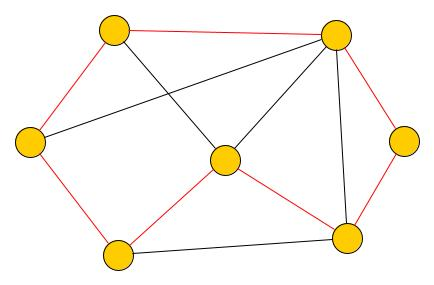
\includegraphics[scale=0.5]{img/graph27}
\end{center}
NP-Complete
\subsection{Eulerian Cycle Problem}
\begin{center}
	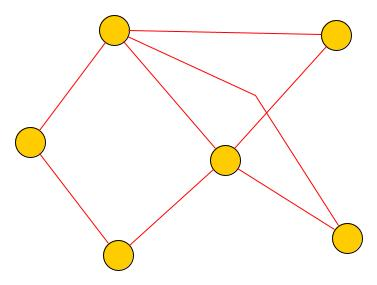
\includegraphics[scale=0.5]{img/graph28}
\end{center}
Cycle exists iff deg(v) is even $\forall v \in V$

($\Rightarrow$): easy, need to go through a vertex (in \& out) $\rightarrow \circ \rightarrow$ \\
($\Leftarrow$): suppose that every vertex has even degree $\Rightarrow$ eulerian cycle observation: 
\begin{center}
	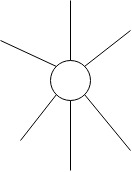
\includegraphics[scale=0.5]{img/vertex1}
\end{center}
take vertex and any two edges and split it into 
\begin{center}
	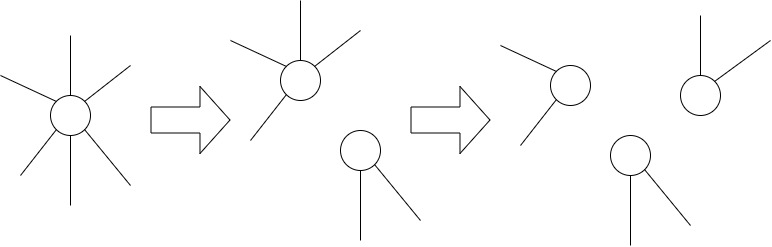
\includegraphics[scale=0.5]{img/vertex2}
\end{center}
$\Rightarrow$ Graph consists of cycles
\begin{center}
	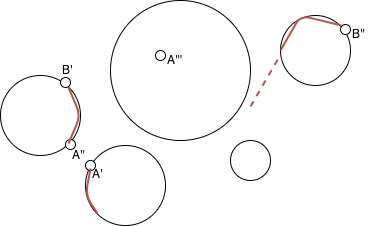
\includegraphics[scale=0.5]{img/vertex3}
\end{center}
construct cycle by arbitrary selecting a node and go along the cycle. If there is a vertex on the way which is a copy of a vertex, go to the next cycle. When a cycle is closed (vertex visited twice) go back. 
\subsection{TSP}
\begin{itemize}
	\item complete graph $K_n$
	\begin{center}
		$n=5:$ 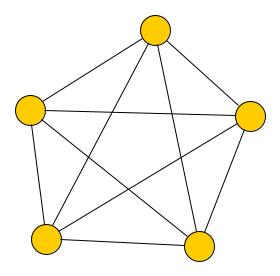
\includegraphics[scale=0.5]{img/graph29}
	\end{center}
	\item weights on the edges
	\item need one with minimum weight
	\item NP complete
\end{itemize}
\subsubsection{Reduction}
There is no construct that can approximate TSP 
$$\nexists \alpha : APP(I) \leq \alpha TSP(I) + \beta$$
"Inapproximability Result" \\
Suppose given a Graph $G$
\begin{center}
	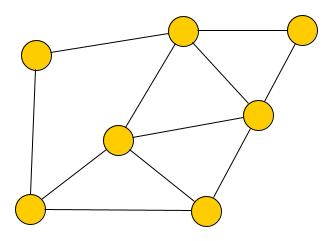
\includegraphics[scale=0.5]{img/graph30}
\end{center}
Specific graph $G \rightarrow K_n$ and weights
\begin{itemize}
	\item add missing edges with $n = |G|$ to get $K_n$
	\item weight of $e$ is, with $G = (V,E), K_n= (V',E')$,
		\begin{itemize}
			\item[1] if $e \in E$ $\forall e \in G \Rightarrow w(e) = 1$
			\item[$\alpha$] if $e \notin E$ $\forall e \notin G \Rightarrow n \cdot \alpha$
		\end{itemize}
	\item[$\Rightarrow$] starting at a problem/instance of the known problem 
	\item[$\Rightarrow$] construct an instance of the problem you want to lower bound
\end{itemize}
Assume we have a $\alpha-$approximation of TSP
\begin{itemize}
	\item[$\Rightarrow$] Hamiltonian Cycle could be solved in polynomial time
	\item[$\Rightarrow$] Hamiltonian Cycle $\in P \lightning$
\end{itemize}
Suppose $\exists$ Hamiltonian Cycle in $G$: $\Rightarrow \exists TSP$ with $cost = n \Rightarrow APP(I) \leq \alpha \cdot n$ \\
Suppose $\nexists$ Hamiltonian Cycle in $G$: $\Rightarrow \forall TSP$ has $cost > \alpha n\Rightarrow APP(I) > \alpha \cdot n$ \\
Metric $TSP$: weights satisfy the triangular inequality (also NP-complete!) \\
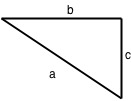
\includegraphics[scale=0.5]{img/tri} $a \leq b + c$ \\
2-approx \\
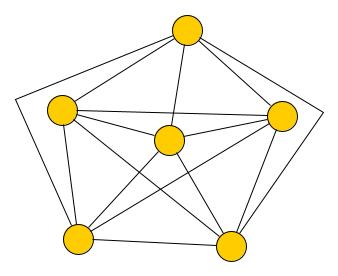
\includegraphics[scale=0.5]{img/graph31} $\stackrel{MST =: T}{\Rightarrow}$ 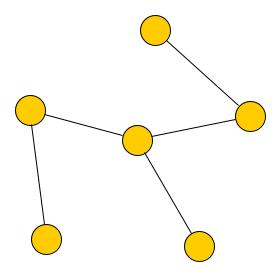
\includegraphics[scale=0.5]{img/graph32} \\
OPT ($=: \alpha$) \\
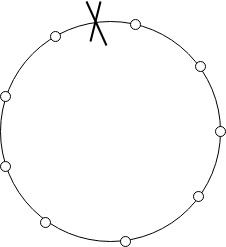
\includegraphics[scale=0.5]{img/st} by removing one edge wer get a spanning tree \\
$cost(T) \leq cost(spanning-path \alpha) < OPT$ \\
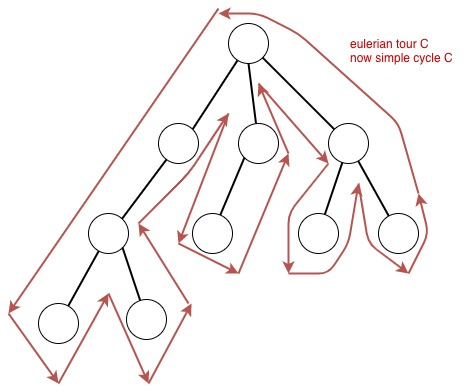
\includegraphics[scale=0.5]{img/cycle1} degree of $v$ gets doubled $\forall v \in V$ 
$$\Rightarrow cost(c) = 2 cost(T)$$
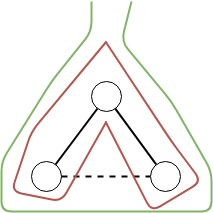
\includegraphics[scale=0.5]{img/cycle2} $C'=$ Hamiltonian Simple Cycle \\
Introduce shortcuts \\ $cost(C')=$? \\
replace the two edges by near one ... $\leq/+/$(triangle inequality!) \\
$cost(C') \leq cost(C)$
$$cost(C') \leq cost(C) = 2cost(T) \leq 2 \cdot OPT$$
Is the analysis tight? \\
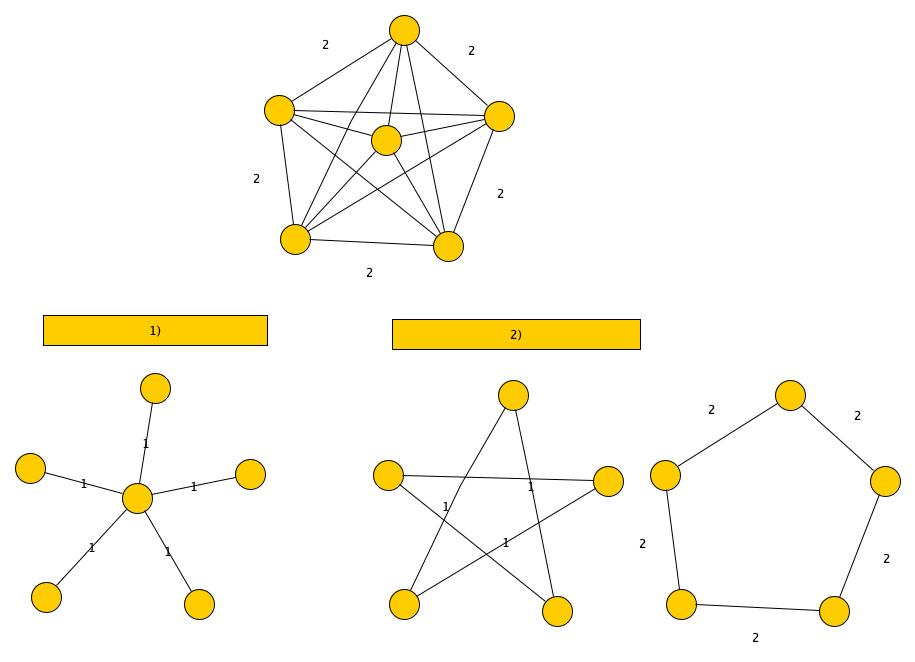
\includegraphics[scale=0.5]{img/graph33}
\subsection{MST}
either 1) or 2) \\
1): \includegraphics[scale=0.5]{img/mst1} $2n-2 \; cost$
\subsection{Christofides}
$$K_n \stackrel{MST}{\rightarrow}T \rightarrow \underbrace{V_0}_{\text{Set of ODD-DEG Vertice}} \stackrel{MIN-COST-PERF.-MATCH}{\longrightarrow} M \rightarrow T \cup M = C \stackrel{SHORTCUT}{\rightarrow} \underbrace{C'}_{hamiltonian \; cycle}$$
Where \\
$K_n$ like before\\
$T$: (E=even, O=odd) \\
\includegraphics[scale=0.5]{img/graph19} \\
We can't have an odd number of vertices with an odd degree
$$\sum_{v \in T}\deg(v) = 2 |E|$$
$$\underbrace{\sum_{v \; ODD}\deg(v)}_{EVEN} + \underbrace{\sum_{v \; EVEN}\deg(v)}_{EVEN} = \underbrace{2 |E|}_{EVEN}$$
\includegraphics[scale=0.25]{img/graph20} All vertices have degree 3/1 ; 
 \includegraphics[scale=0.25]{img/graph21} All vertices have degree 2 except 2 \\
 $M$: \\
 \includegraphics[scale=0.25]{img/graph22} Perfect Matching (red) (even number of vertices $\rightarrow \exists$ perfect matching) with Min-Cost \\
 $T \cup M$: \\
 1. red (even vertices?), 2. green (perfect match): \includegraphics[scale=0.25]{img/graph23} \\
 \begin{align*}
 	cost(C') &\leq cost(C) & |\text{triangle inequality}\\
 	cost(C) &= cost(T) + cost(M) & |cost(T) < OPT,(*)  \\
 	cost(C_o^*) &\leq OPT & | (*1)	\\
 	(cost(M) \leq)cost(M^*) &\leq \frac{cost(C_0^*)}{2} & |cost(M) \leq \frac{OPT}{2} \\
 	cost(T) + cost(M) \leq \frac{3}{2}OPT
 \end{align*}
$$(*) C_0^* = \text{cycle derived from $C^*$ but only odd degree vertices}$$
$$(*1) \text{There are 2 perf. match. in } C_0^*, \text{take the minimal } M^*$$
We have everything we want, but we don't know whether we can do better or not. The best bound known is $\frac{3}{2}OPT$. Example that gets $\frac{3}{2}OPT$: (all edges without cost have cost 1, missing edges are very very expensive) \\
\includegraphics[scale=0.25]{img/graph24}
\\ OPT ($cost = n$): \\ \includegraphics[scale=0.25]{img/graph25} \\
Consider the red $MST$ is found: \\ \includegraphics[scale=0.25]{img/graph26},\\ the perfect matching would include the n/2 edge that leads to a cycle. The cost is $n-1$ for the tree and $\frac{n}{2}$ for the edge. So: $\frac{3}{2}n$ \\
On the n/2 you can't put something greater than $\frac{n}{2}$ because of the triangle inequality. 
\subsection{PTAS: Polynomial Time Approximation Schema}
Schema: Not one approximation but an algorithm with a parameter. Balance between complexity and accuracy. \\
$\varepsilon > 0$ \\
Approx $\underbrace{(1 + \varepsilon)}_{Minimization}$ or $\underbrace{(1- \varepsilon)}_{Maximazation}$ \\
Time depends on $\frac{1}{\varepsilon}$ and $n$, possible approx.: $\underbrace{\mathcal{O}(n^{\frac{1}{\varepsilon}})}_{PTAS}$, much better: $\underbrace{\mathcal{O}(\frac{1}{\varepsilon}n)}_{F(ully)PTAS}$ 
\subsubsection{Knapsack}
\paragraph{Input}
$a_1,...,a_n$ items, each item has a size $s(a_i)$ and a profit $P(a_i)$. \\
Bag $B$ with a capacity $c(B)$
\paragraph{Output} Set of item $S$ that fits in the bag: 
$\sum_{a_i\in S}s(a_i) \leq c(B)$ and
maximize $\sum_{a_i \in S}P(a_i)$

simpler: $(\notin NP)$ raking functions of items \\
$A(i,P)$: smallest subset of the first $i$ items whose profit is equal to $P$ \\
Try to compote the first (specific value of a profit $\in \{1...\}$) $i$ items Knapsack, continue to $i+1 \in \{1...n\}$

Example: \\
\begin{tabular}{c|c|c}
& $s(a_i)$ & $P(a_i)$ \\ \hline 
$a_1$ & 3 & 20 \\
$a_2$ & 5 & 32 \\
$a_3$ & 4 & 40 \\
$a_4$ & 1 & 28 \\
$a_5$ & 2 & 20 \\
\end{tabular} \\
$A(5,100)$: \\
$a_2,a_3,a_4 \rightarrow P = 100, s = 10$ \\
$a_1,a_2,a_4,a_5 \rightarrow P = 100, s = 11$ \\
$A(5,99) = \infty$ \\
\begin{tabular}{cccccc|c|}
	& $i \rightarrow $ & 1 & 2 & 3 & ... & n \\
	& 1 & $\infty$ & $\infty$ & & & \\
	& 2 & $\infty$ & $\infty$ & & & \\
	& 3 & $\infty$ & $\infty$ & & & \\
	& ... & ... & ... & & & \\
	20 & ... & 3 & 3 & & & $\leq B$ \\
	& ... & ... & $\infty$ & & &  \\
	32 & ... & ... & 5 & & &  \\
	& ... & ... & $\infty$ & & &  \\
	52 & ... & ... &85 & & &  \\
	& ... & ... & $\infty$ & & &  \\
	& n & $\infty$ & ... & && \\
	& $\uparrow$ &&&&& $\uparrow$ \\
	& $P$ &&&&& \\
\end{tabular} \\
$$A(i,P) = \begin{cases}
s(a_i) + A(i-1,P-P(a_i)) & use \; i \\A(i-1,P) & don't \; use \; i
\end{cases}$$
stop at $A(n,n \cdot \underbrace{P_M}_{max \; profit \; of \; an \; item})$ $\rightarrow$ Solution $S$ cannot get better! \\
then read the table (last column) \\
complexity: $\#cells$, $\mathcal{O}(n\cdot n \cdot P_M) = \mathcal{O}(n^2 \cdot P_M)$ \\
$P_M$ is problem, because $P_M$ is a number $\Rightarrow$ represented in logarithmic number of bits $\Rightarrow$ input $\log$ $\Rightarrow$ output exonential ($\Rightarrow\in NP$) in terms of input. \\
$$ K = \frac{\varepsilon \cdot P_M}{n} \Rightarrow P^*(a_i) = \lfloor \frac{P(a_i)}{K} \rfloor $$
obtain complexity: $$\mathcal{O}(n^2 \cdot P_M^*) = \mathcal{O}(n^2 \cdot \lfloor \frac{P_M}{\underbrace{\varepsilon \cdot P_M}_{n}} \rfloor
) = \mathcal{O}(\frac{n}{\varepsilon})$$
$S^*$ set computed on the star instance \\
know: $S^* = OPT^*$ \\
compare to: $OPT = S_0$
$$\frac{P(a_i)}{K}-1 \leq P^*(a_i) \leq \frac{P(a_i)}{K} (da \lfloor\rfloor )$$
\begin{align*}
	&P(a_i) - K P^*(a_i) \leq K \forall i \\
	&\stackrel{\sum_{S_0}}{\Rightarrow} \underbrace{\sum_{a_i \in S_0}(P(a_i) - KP^*(a_i))}_{P(S_0) = KP^*(S_0) \leq K_n} \\
	& \leq K|S_0| \leq K_n \\
	P(S^*) &\leq KP^*(S^*) \geq K\underbrace{P^*(S_0)}_{\text{just some solution in $P^*$ and $S^* = OPT$}} \geq P(S_0) - K_n \geq OPT - K_n \\
	&= OPT - \varepsilon P_M \stackrel{P_M \leq OPT}{\geq} OPT - \varepsilon OPT \\
	&= (1 - \varepsilon) \cdot OPT
\end{align*}
\subsubsection{Bin Packing}
\paragraph{Input} $a_1,...,a_n$ items with sizes $s(a_1),...,s(a_n)$, $\forall i s(a_i) \leq 1$. No profits. We want to fit all items in a certain number of bins. We have maximal $n$ bins (every item one bin), but want minimal number of bins. Bin-size is 1.
\paragraph{Output} Configuration to fit $a_1,...,a_n$ in minimal number of bins. \\
to be continued ...
\subsubsection{2-Partition}
Strong related to Bin Packing (pack items in two bags). 
\paragraph{Input} $i_1,...,i_n$ Integers
\paragraph{Output} Partition of $i_1,...,i_n$ in two partitions $I_1,I_2$ with $$\sum_{i \in I_1}i = \sum_{i \in I_2}i$$

Reduction between these two problems 2-Partition $\leq$ Bin Packing: Positive instance $i_1,...i_n$ means they fit into 2 bins, else they don't. 

\paragraph{Approximation}
The approximation is $\frac{3}{2}$ (positive instance). There is no $\alpha \leq \frac{3}{2}$. \\
PTAS: $(1+\varepsilon) \rightarrow$ PTAS doesn't exist (inaproximability) $\Rightarrow$  APTAS

\subsection{APTAS}
Asymptotic PTAS. Look at large instances $\Rightarrow \frac{n+1}{n} \frac{n (1+\frac{1}{n})}{n} \rightarrow 1$ \\ 
$$ALG(I) \leq (1+ \varepsilon)OPT + C$$
Add a constant $C$ to handle extreme cases in small instances

\subsubsection{Bin Packing (continuation)}
Greedy approach
\begin{itemize}
	\item $a_1$ in $bin_1$
	\item $a_2$: does it fit in $bin_1$? yes: put it in $bin_1$, else in $bin_2$ (then $bin_1$ is closed)
	\item $a_3$: does it fit in the current? ...
\end{itemize}
$\Rightarrow$ try to fit it into the current bin, if it doesn't fit, got to the next bin. \\ \newline 
Optimal solution: all bins are completely full $\Rightarrow OPT \; bins \Rightarrow \sum i = OPT$ \\
There could be $bin$s that are nearly empty, because the next item doesn't fit in the bin, so the bin stays nearly empty (even if there were other items that fit in). \\
Connect $bin_1,bin_2$ and $bin_3,bin_4$,.... For each pair the sum is $>1$ and $\leq 2$. $\Rightarrow$ Approximation with factor 2. \\ 
\paragraph{APTAS} instance $I$: $1,3,3, 5, 6, 6, 8, 10, 12, 14$. Select $\varepsilon = 4$ \\ \newline 
$\underbrace{1,3,3}_{small (<4)} | \underbrace{5, 6, 6, 8, 10, 12, 14,16}_{large}$ \\ \newline 
$I_L = \underbrace{5,6,6}_{=\frac{|I_L|}{k}},\underbrace{8,10,12}_{=\frac{|I_L|}{k}},\underbrace{14,16}_{\leq\frac{|I_L|}{k}}$, bin capacity $c$, items $\geq \varepsilon \rightarrow  \frac{c}{\varepsilon}$ items maximal \\ \newline  
$I_L':6,6,6 | 12,12,12 | \times$ $$\Rightarrow ALG(I_L') \stackrel{brute-force}{=}OPT(I_L')$$ \\
Now: $ALG(I_L') \rightarrow ALG(I_L) \rightarrow ALG(I)$ and how does it change the relationship to $OPT(I_L), OPT(I)$ \\ \newline 
$ALG(I_L') \rightarrow ALG(I_L)$: Split $I_L'$ to the bins. Replace the Element by their real value (works because they just got greater in $I_L'$). The last group $\times$ just gets a bin for each item. $$ALG(I_L) \leq ALG(I_L') + \frac{|I_L|}{k}$$
$OPT(I_L) \rightarrow OPT(I_L')$ The last element in the first $I_L'$ group is smaller than the first in the next group in $I_L$. So every group in $I_L'$ can be mapped to the next group in $I_L$. The last group of $I_L$ remains . \\
We have an optimal solution for $I_L$ given. Cut the elements of the first group. replace group 2 elements of $I_L$  by group 1 elements of $I_L'$. In the example: replace in $OPT$-solution: $8,10,12$ by $6,6,6$. \\
\begin{center}
\includegraphics[scale=0.5]{img/bin-pack} 
\end{center}
$$OPT(I_L') \leq OPT(I_L)$$
$$ALG(I_L) \leq ALG(I_L') + \frac{|I_L|}{k} = OPT(I_L') + \frac{|I_L|}{k} \leq OPT(I_L) + \frac{|I_L|}{k}$$
Chosse $k = \frac{1}{\varepsilon^2}$. The following holds: $OPT(I_L) \geq \sum sizes \geq |I_L|\varepsilon$. So:
$$ OPT(I_L) + \frac{|I_L|}{k} = OPT(I_L) + |I_L|\varepsilon^2 \leq OPT(I_L) + OPT(I_L) \cdot \varepsilon  = (1+ \varepsilon) OPT(I_L)$$
$$\Rightarrow ALG(I_L) \leq (1+\varepsilon)OPT(I_L)$$
Now we want to go back to the initial instance. So we need to put the small item somewhere. For that use the greedy approach and just fill the gaps.
\begin{enumerate}
	\item All small elements fit in the gaps $\Rightarrow ALG(I) = ALG(I_L) \checkmark$, we are ok
	\item Otherwise: We need extra bin(s). If they don't fit create a new bin and try to fit them there. If this is full get a new one and so on. But there are still gaps in the bins before. There can't be any elements greater than $\varepsilon$ (they are filled by $1-\varepsilon$ if the capacity is 1).
	$$(ALG(I)-1) \cdot (1-\varepsilon) \leq \sum sizes \leq OPT(I)$$
	$$ALG(I) \leq \frac{OPT(I)}{1-\varepsilon}+1$$
	(The 1 (=$C$) defines the APTAS) \\
	for $\varepsilon \leq \frac{1}{2} \rightarrow 1 + 2 \varepsilon$
		$$ALG(I) \leq \frac{OPT(I)}{1-\varepsilon}+1 \leq (1+2\varepsilon)OPT(I) + 1$$
\end{enumerate}
	\section{Linear Programming}

\subsection{Problem}
A factory produces tables and chairs
\begin{itemize}
	\item 1 table requires 1 unit of metal and 3 units of wood
	\item 1 chair requires 2 units of metal and 1 unit of wood
	\item The factory has 600 units (900 units) of metal (wood)
	\item The profit of 1 table is 100\EUR and 1 chair is 100\EUR
\end{itemize}
\paragraph{Question} How many tables/chairs to produce to maximize the profit?
$$x_1: \#tables \; to \; produce \Rightarrow x_1 \geq 0$$
$$x_2: \#chairs \; to \; produce \Rightarrow x_2 \geq 0$$
\paragraph{Profit} $100(x_1+x_2) = 100 x_1 + 100 x_2$
\paragraph{Constraints} $x_1 + 2x_2 \leq 600$ and $3x_1+x_2 \leq 900$
\paragraph{Maximize}  \textcolor{green}{$100x_1+100x_2$} 
\paragraph{Subject to (s.t.)} \textcolor{yellow}{$x_1 + 2x_2 \leq 600$} and \textcolor{orange}{$3x_1+x_2 \leq 900$} and \textcolor{blue}{$x_1,x_2 \geq 0$} \\
\begin{center}
	\includegraphics[scale=0.75]{img/dia1}
\end{center}
$$100x_1+100x_2 = 30000 (x_1=0,x_2 = 300 \equiv x_1 = 900, x_2=0)$$
\paragraph{Observation} As the line $100x_1+100x_2=c$ moves toward $P$, the profit gets increased. $\Rightarrow$ $P$ is optimal (intersection of $\stackrel{(1)}{x_1}+2x_2=600$, $3x_1+\stackrel{(2)}{x_2} = 900$) \\
\begin{itemize}
	\item[(1)] $\Rightarrow x_1 = 600 - 2x_2$
	\item[(2)] \begin{align*} &\stackrel{(1)}{=}2(600-2x_2)+x_2 = 900 \\
	& 1800 - 6x_2+x_1 = 900 \\
	&5x_2 = 900 \Rightarrow x_2 = 180
	& \Rightarrow x_1 = 240
	\end{align*}
\end{itemize}
\paragraph{Optimal} $x_1 = 240, x_2 = 180$
\paragraph{Profit} 42000 \EUR
\paragraph{Different cases}
\begin{center}
	\includegraphics[scale=0.5]{img/dia3}
\end{center}
(a),(b) $\Rightarrow$ bounded feasible solution $\Rightarrow \exists$ solution $\Rightarrow$ corner solution \\
(c) $\Rightarrow$ feasible (corner solution) or infeasible/unbounded
$$\text{(a),(b),(c)} \exists solution \Rightarrow \exists corner solution$$
\begin{itemize}
	\item[(1)] bounded feasible (a),(b)
	\item[(2)] unbounded feasible (c) min
	\item[(3)] unbounded infeasible (c) max
	\item[NOT] \sout{un}bounded infeasible
\end{itemize}

\subsubsection{Generalization}
\paragraph{Maximize} $c_1x_1 + c_2x_2 + ... + c_nx_n \rightarrow$ objective function (linear)
\paragraph{Minimize} \phantom, 
\paragraph{Subject to} constraints set \\
\begin{center}
\begin{tabular}{c|c|c}
	& one-of & \\
	$a_{11}x_1+a_{12}x_2+...a_{1n}x_n$ &  & $b_1$ \\ 
	& $\leq$ & \\
	$a_{21}x_1+a_{22}x_2+...a_{2n}x_n$ & & $b_2$ \\
	& $=$ & \\
	... & & ... \\
	& $\geq$ & \\
	$a_{m1}x_1+a_{m2}x_2+...a_{mn}x_n$ & & $b_m$ \\
\end{tabular}
\end{center}
optional non-negativity constraint: $(x_1,x_2,...,x_n \geq 0)$ 

\subsection{Another example: Max-flow}
\paragraph{Input} directed graph $G=(V,E),s,t \in V$ \\
$indegree(s) = outdegree(t) = 0$ \\
capacities $c: E \rightarrow \mathbb{R}^+$
\paragraph{Output} find $f: E \rightarrow \mathbb{R}^+$ such that:
\begin{itemize}
	\item[(1)] $\forall(u,v) \in E: 0 \leq f(u,v) \leq c(u,v)$
	\item[(2)] $\sum_{(u,v) \in E}f(u.v) = \sum_{(v,u) \in E}f(u,v) \forall u \in V-{s,t}$
	\item[(3)] $max \sum_{(s,v) \in E}f(s,v)$
\end{itemize}
\subsubsection{LP formulation}
maximize $\sum_{(s,v) \in E}f(s,v)$ (3) \\
s.t.
\paragraph{Constraints} $f(u,v) \leq c(u,v) \forall (u,v) \in E (\approx 1)$ \\
$\sum_{(u,v) \in E}f(u.v) = \sum_{(v,u) \in E}f(u,v) \forall u \in V-{s,t}$ (2)
\paragraph{Negativity} $f(u,v) \geq 0 \forall (u,v) \in E$ 

\subsubsection{Geometric representation in higher dimensions}
\begin{center}
	\includegraphics[scale=0.5]{img/dia2}
\end{center}
Simplex: Move from corner to corner

\subsection{Standard form}
\paragraph{Maximization} $c_1x_1 + c_2x_2 + ... + c_nx_n$
\paragraph{Subject to} \begin{align*}
	a_{11}x_1 + a_{12}x_2  + ... + a_{1n}x_n  &\leq b_1 \\
	a_{21}x_1 + a_{22}x_2  + ... + a_{2n}x_n  &\leq b_2 \\
	... \\
	a_{m1}x_1 + a_{m2}x_2  + ... + a_{mn}x_n  &\leq b_m \\
	x_1,x_2,...,x_n  &^\geq 0 \\
\end{align*}
\paragraph{Maximization} $C^Tx$
\paragraph{Subject to} \begin{align*}
	Ax &\leq b \\
	x & \geq 0
\end{align*}
$$C = \begin{bmatrix}
c_1 \\ c_2 \\ ... \\ c_n
\end{bmatrix} \Rightarrow C^T = \begin{bmatrix}
c_1,...,c_n
\end{bmatrix}$$
$$x_1 = \begin{bmatrix}
x_1 \\ x_2 \\ ... \\ x_n
\end{bmatrix} \hspace*{1cm} b = \begin{bmatrix}
b_1 \\ ... \\ b_m
\end{bmatrix} \hspace{1cm} A = \begin{bmatrix}
a_{11} & a_{12} & ... & a_{1n} \\
a_{21} & a_{22} & ... & a_{2n} \\
... \\
a_{m1} & a_{m2} & ... & a_{mn} 
\end{bmatrix}$$
First step of (pre-processing) simplex to bring the input LP to the standard form.

Why not in standard form?
\begin{itemize}
\item[(1)] minimize $c_1x_1+c_2x_2+...+c_nx_n \Leftrightarrow$ maximize $-c_1x_1-c_2x_2-...-c_nx_n$
\item[(2)] Equality $a_{j1}x_1 + a_{j2}x_2 + ... + a_{jn}x_n = b_j$ \\ $\Leftrightarrow a_{j1}x_1 + a_{j2}x_2 + ... + a_{jn}x_n \leq b_j$ \\
$\& (-) a_{j1}x_1 +(-) a_{j2}x_2 +(-) ... +(-) a_{jn}x_n \geq (\leq) b_j$
\item[(3)] $\geq$ inequality $a_{j1}x_1 + a_{j2}x_2 + ... + a_{jn}x_n \geq b_j \Leftrightarrow -a_{j1}x_1 - a_{j2}x_2 - ... - a_{jn}x_n \leq -b_j$
\item[(4)] Absence of non-negativity constraints.
\end{itemize}
Replace: \\ 
$x_j \rightarrow x_j' \& x_j''$ \\
$x_j = x_j'-x_j'';x_j',x_j'' \geq 0$
\paragraph{Example} ~ \\
\begin{tabular}{ccccc}
minimize& $-2x_1+3x_2$ && maximize &$2x_1-3x_2'+3x_2''$ \\
s.t. & \textcolor{red}{$x_1+x_2 = 7$} && s.t. & $x_1+x_2'-x_2'' \leq 7$ \\
& $x_1-2x_2 \leq 5$ & $\rightarrow$ && $-x_1-x_2'+x_2'' \leq -7$ \\
& $x_1 \geq 0$ &&& $x_1-2x_2''+2x_2'' \leq 5$ \\
&&&& $x_1,x_2',x_2'' \geq 0$ \\
\end{tabular} \\
\textcolor{red}{non-negativity for $x_1=x_2'-x_2''$}

\subsection{The simplex method}

\subsubsection{By an example}
\begin{align*}
\text{maximize } & 5x_1+4x_2+3x_3 \\
\text{s.t. } & 2x_1+3x_2+x_3 \leq 5 \\
\text{(in standard }  & 4x_1 + x_2 + 2x_3 \leq 11 \\
\text{form) } & 3x_1 + 4x_1 + 2x_3 \leq 8 \\
& x_1,x_2,x_3 \geq 0
\end{align*}
\begin{itemize}
\item[(1)] Introduce a name for the objective function 
$$J = 5x_1+4x_2+3x_3$$
\item[(2)] Introduce a slack (difference between right and left) variable for each constraint
$$x_4 = 5-2x_1-3x_2-x_3 ; x_4 \geq 0$$
$$\text{right-left side $\geq 0 \Rightarrow$ right-left side $=x_4, x_4 \geq 0$}$$
\end{itemize}
Standardform $\rightarrow$ slack form
\begin{align*}
\text{maximize} J &= \textcolor{orange}{5x_1 + 4x_2 + 3x_3} \\
\textcolor{green}{x_4} &= 5-\textcolor{orange}{2x_1-3x_2-x_3} (1) \\ 
\textcolor{green}{x_5} &= 11-\textcolor{orange}{4x_1-x_2-2x_3}  (2) \\
\textcolor{green}{x_6} &= 8-\textcolor{orange}{3x_1-4x_2-2x_3}  (3) \\
x_1,x_2,x_3,x_4,x_5,x_6 \geq 0
\end{align*}
\textcolor{green}{non-zero variables}, \textcolor{orange}{zero variables}
\paragraph{Idea} Start with a solution $(x_1,x_2,x_3,x_4,x_5,x_6)$, dinf another solution $(\overline{x_1},\overline{x_2},\overline{x_3},\overline{x_4},\overline{x_5},\overline{x_6})$ s.t, iterate $5x_1+4x_2+3x_2 \leq 5\overline{x_1} + 4\overline{x_2} + 3\overline{x_3}$
\paragraph{Problem} Initial feasible solution to start the iteration? \\
In the example: Easy! $x_1=x_2=x_3=0.x_4=5,x_5=11,x_6=8,J=0$
\paragraph{Assumption} $b_1,b_2,...,b_n \geq 0 \Rightarrow x_1 = x_2 = ... = x_n = 0$ is feasible \\
How can we find a better solution than $J=0$?
\paragraph{Observation} If we increase $x_1$ (or $x_2$ od $x_3$) (positive coefficient), then $J$ will also increas, but we must ensure that $x_4,x_5,x_6 \geq 0$ \\
Since $x_2=x_3 = 0$
\begin{itemize}
	\item $x_4 \geq 0 \Rightarrow 5-2x_1 \geq 0 \Leftrightarrow x_1 \leq \frac{5}{2}= 2.5$
	\item $x_5 \geq 0 \Rightarrow 11-4x_1 \geq 0 \Leftrightarrow x_1 \leq \frac{11}{4} = 2.75$ 
	\item $x_6 \geq 0 \Rightarrow 8 -3x_1 \geq 0 \Leftrightarrow x_1 \leq \frac{8}{3}= 2.66...$
\end{itemize}
New solution: $x_1 = \frac{5}{2}, x_2,x_3 = 0, x_4 = 0, x_5 = 1, x_6 = \frac{1}{2} J = \frac{25}{2} = 12.5$ \\
How do we proceed? 
\paragraph{Observation} THe first step was easy beacuse all non-zero variables were expected as linear combination of zero variables ($x_1$ now got non zero).
\begin{itemize}
	\item (1) $\Leftrightarrow 2x_1 = 5-3x_2 -x_3-x_4 \Leftrightarrow x_1 = \frac{5}{2} - \frac{3}{2}x_2 - \frac{1}{3}x_3 - \frac{1}{2}x_4$
	\item $J=5(\frac{5}{2} - \frac{3}{2}x_2 - \frac{1}{3}x_3 - \frac{1}{2}x_4) + 4x_2 + 3x_3 \Leftrightarrow J = \frac{25}{2} - \frac{7}{2}x_2 + \frac{1}{2}x_3 - \frac{5}{2}x_4$
	\item $x_5 = 11 - 4 (\frac{5}{2} - \frac{3}{2}x_2 - \frac{1}{3}x_3 - \frac{1}{2}x_4) - x_2 - 2x_3 \Leftrightarrow x_5 = 1 + 5x_2 + 2x_4$
	\item $x_6 = 8-3(\frac{5}{2} - \frac{3}{2}x_2 - \frac{1}{3}x_3 - \frac{1}{2}x_4) - 4x_2 - 2x_3 \Leftrightarrow x_6 = \frac{1}{2} + \frac{1}{2}x_2 - \frac{1}{2}x_3 + \frac{3}{2}x_4$
\end{itemize}
maximize $J = \frac{25}{2} - \frac{7}{2}x_2 + \frac{1}{2}x_3 - \frac{5}{2}x_4$
\begin{align*}
x_1 &= \frac{5}{2} - \frac{3}{2}x_2 - \frac{1}{3}x_3 - \frac{1}{2}x_4 \\
x_5 &= 1 + 5x_2 + 2x_4 \\
(*)x_6 &= \frac{1}{2} + \frac{1}{2}x_2 - \frac{1}{2}x_3 + \frac{3}{2}x_4 \\
&x_1,...,x_6 \geq 0. x_1,x_5,x_6 \text{ non zero variables}
\end{align*}
\paragraph{Observation} If we increase $x_2$ or $x_4$, then $J$ will decrease (bad idea), so we have to increase $x_3$ (positive coefficient) \\
Since $x_2=x_4 = 0$: \\
\begin{itemize}
	\item $x_1 \geq 0 \Leftrightarrow \frac{5}{2}-\frac{1}{2}x_3 \geq 0 \Leftrightarrow x_3 \leq 5$
	\item $x_5$ does not relate $x_3 \Rightarrow$ not constrained
	\item $x_6 \geq 0 \Leftrightarrow \frac{1}{2}x_3 \geq 0 \Leftrightarrow x_3 \leq 1$
\end{itemize}
New soluion: $x_1 = 2, x_2 = 0, x_3 = 1, x_4 = 0, x_5 = 1, x_6 = 0$ \\
maximize $J = 13 - 3x_2 - x_4 - x_6$ \\
\begin{align*}
\text{s.t. } x_3 &= 1 + x_2 + 3x_4 - 2x_6 (*) \\
x_1 &= 2 - 2x_2 - 2x_4 + x_6 \\
x_5 &= 1 + 5x_2 + 2x_4 \\
&x_1,x_2,...,x_6 \geq 0
\end{align*}
If $x_2,x_4,x_6$ are increased, then $J$ decreases $\Rightarrow J$ is optimal. 
\begin{enumerate}
	\item The last system is equivalent to the first
	\item In the last system all variables must be non-zero (cant't decrease variable to $<0$ e.g. $13-3\cdot(-2) \lightning x_2 \geq 0$!)
\end{enumerate}	

\subsubsection{Theory}
\begin{itemize}
	\item Preprocessing step: general LP $\stackrel{rules}{\rightarrow}$ LP in standard form. 
	\item Assumption
	\begin{enumerate}
		\item maximize $c_1x_1+c_2x_2+...+c_nx_n$ \\
		s.t. $a_{j1}x_1+a_{j2}x_2+...a_{jn}x_n \leq bj \forall j=1,2,...,m$ \\
		$x_i \geq 0 \forall i = 1,2,...,n$
		\item $b_1,...,b_m \geq 0 \Rightarrow x_1=x_2=...=x_n=0$ is feasible.
	\end{enumerate} 
\end{itemize}
Transform to Slack Form: \\
maximize $J = \sum_{i=1}^nc_1x_i$ (Initial Dictionary)\\
s.t. $x_{n+1} = b_j - \sum_{i=1}^na_{ji}x_i \forall j = 1,...,m$ \\
$x_1 \geq 0 \forall i = 1,...,n+m$ \\
$x_{n+1}$ are slcak variables. \\
zero-value variables ($x_1 \forall i = 1,...,n$)$\rightarrow$ non-basic.\\
non-zero-value variables ($x_i \forall i = n+1,...,n+m$) $\rightarrow$ basic. \\
At every step of the simplex
\begin{itemize}
	\item one basic variable becomes non-basic
	\item one non-basic variable becomes basic
\end{itemize}
At some step of the simplex: \\
$B$: the set of indices of the basic variables \\
$N$: the set of indices of the non-basic variables \\
maximize $J = \underbrace{\overline{J}}_{\text{value of obj. funciton}} + \sum_{i \in N}\overline{c}_ix_i$ \\
s.t. $x_i = \overline{b}_i - \sum_{j \in N}\overline{a_{ij}}x_j \forall i \in B$ \\
$x_i \geq 0 \forall i \in B \cup N$ 
\paragraph{Entering variable}  Is one in $N^+ = \{x_i, \overline{c_i}>0 i \in N\}$ (if $x_i$ is increased, then $J$ is increased)
\begin{itemize}
	\item $N^+ = \emptyset \Rightarrow J = \overline{J}$ is optimal (since increasing any of the non-basic variables will decrease $J$)
	\item $|N^+| > 1$: select the entering variable as the one with the smalles index. 
	\item[$\Rightarrow$] let $x_k$ be the entering variable.
\end{itemize}
\paragraph{Exiting variable} We have to ensure that all basic variables $x_i \geq 0 \forall i \in B \stackrel{\forall i \in N  -\{k\} x_i = 0}{\Longrightarrow}$ \\
$$\Leftrightarrow \overline{b_i} - \sum_{j \in N}\overline{a_{ij}}x_j \geq 0 \forall i \in B$$ 
$$\Leftrightarrow \overline{b_i} - \overline{a_{ik}}x_k \geq 0 \forall i \in B$$ 
$$\stackrel{a_{ik}>0 \lor a_{ik}<0}{\Longleftrightarrow} \begin{cases}
x_k \leq \frac{\overline{b_i}}{\overline{a_{ik}}} & a_{ik} > 0 \\
x_k \geq \frac{\overline{b_i}}{\overline{a_{ik}}} & a_{ik} < 0\\
\end{cases}$$
We chose the exiting variable as the one for which $\frac{\overline{b_i}}{a_{ik}}$ is minimum and $a_{ik} > 0$ \\
\fbox{\parbox{\linewidth}{Note: If $\overline{a_{ik}}<0$, there is no restriction on how much we can increase $x_k \Rightarrow$ the System is unboundes and $J \rightarrow + \infty$}} 

\subsection{Duality}
Each LP (original/primal LP) has an associated, called dual, LP.
\paragraph{Origninal LP (standard form)} $n$ variables, $m$ constraints \\
\begin{align*}
\text{maximize } & c_1x_1+c_2x_2+...+c_nx_n \\
\text{s.t. } &a_{11}x_x+a_{12}x_2+...+a_{1n}x_n \leq b_1 \\
&... \\
&a_{m1}x_1+a_{m2}x_2+...+a_{mn}x_n \leq b_m \\
&x_1,...,x_n \geq 0
\end{align*}
\paragraph{Dual LP (standard minimal form)} $m$ variables, $n$ constraints \\
\begin{align*}
\text{minimize } & b_1y_1+b_2y_2+...+b_my_m \\
\text{s.t. } &a_{11}y_x+a_{21}y_2+...+a_{m1}y_m \geq c_1 \\
&... \\
&a_{1n}y_1+a_{2n}y_2+...+a_{mn}y_m \geq c_n\\
&y_1,...,y_m \geq 0
\end{align*}
\paragraph{Primal} ~ \\
\begin{align*}
\text{maximize } &c^Tx \\
\text{s.t. } & Ax \leq b \\
& x \geq 0
\end{align*}
$$c = \begin{bmatrix}
c_1 \\ c_2 \\ ... \\ c_n
\end{bmatrix} \Rightarrow C^T = \begin{bmatrix}
c_1,...,c_n
\end{bmatrix}$$
$$x = \begin{bmatrix}
x_1 \\ x_2 \\ ... \\ x_n
\end{bmatrix} \hspace*{1cm} b = \begin{bmatrix}
b_1 \\ ... \\ b_m
\end{bmatrix} \hspace{1cm} A = \begin{bmatrix}
a_{11} & a_{12} & ... & a_{1n} \\
a_{21} & a_{22} & ... & a_{2n} \\
... \\
a_{m1} & a_{m2} & ... & a_{mn}
\end{bmatrix} \hspace*{1cm} y = \begin{bmatrix}
y_1 \\ y_2 \\ ... \\ y_m
\end{bmatrix}
$$
\paragraph{Dual} ~ \\
\begin{align*}
\text{minimize } &c^Tx \\
\text{s.t. } & yA \geq c^T \\
& y \geq 0
\end{align*}
\begin{center}
\begin{tabular}{c|cccc|c}
& $x_1$ & $x_2$ & ... & $x_n$ & \\ \hline 
$y_1$ & $a_{11}$ & $a_{12}$ & ... & $a_{1n}$ & $\leq b_1$ \\
$y_2$ & $a_{21}$ & $a_{22}$ & ... & $a_{2n}$ & $\leq b_2$ \\
... & ... & ... &...& ...& ... \\
$y_n$ & $a_{m1}$ & $a_{m2}$ & ... & $a_{mn}$ & $\leq b_m$ \\ \hline 
& $\geq c_1$ & $\geq c_2$ & ... & $\geq c_n$ & \\
\end{tabular} 
\end{center}
1. equation of dual: $y$ columns and the $x_1$ column. \\
1. equation of orimal: $x$ row and $y_1$ row
\begin{align*}
\text{maximize } &100x_1 + 100x_2 \\
\text{s.t. } &x_1+2x_2 \leq 600 \\
&3x_1+x_2 \leq 900 \\
x_1,x_2 \geq 0
\end{align*}
Dual:
\begin{align*}
\text{minimize } &600y_1+900y_2 \\
\text{s.t. } &y_1+3y_2 \geq 100 \\
&2y_1+y_2\geq 100 \\
y_1,y_2 \geq 0 
\end{align*}

\subsubsection{Weak duality theorem}
If $x = [x_1,...,x_n]^T$ is a feasible solution of the primal \\
and $y = [y_1,...,y_n]^T$ is a feasible solution of the dual \\
$\Rightarrow c^T \leq y^Tb$ \\
Any feasible solution of the primal is upper bounded by any feasible solution of the dual.
\paragraph{Proof} $x$ is feasible in the primal $\Rightarrow Ax \leq b; x \geq 0 \stackrel{ (y^T*)\geq 0}{\Rightarrow} \textcolor{red}{y^TAx} \leq y^Tb$ \\
$y$ is feasible in the dual $\Rightarrow yA \geq c; y \geq 0 \stackrel{\cdot (*x) \geq 0}{\Rightarrow} \textcolor{red}{y^TAx} \geq c^Tx$ 
$$\Rightarrow c^Tx \leq y^TAx \leq y^Tb	$$
$$\underbrace{-------------op}_{primal \; values}---------\underbrace{od-------------}_{dual \; values}$$
op = optimal primal value, od = optimal dual value \\
Is there a Gap between op and od? $\stackrel{Strong \; duality \; theorem}{\longrightarrow}$ $\nexists$ Gap

\paragraph{Corollary} If $x,y$ are feasible for the primal and the dual s.t. $c^Tx = y^Tb$, then $x\&y$ are optimal.
\end{document}